\documentclass[11pt]{article}
\usepackage{geometry}                
\geometry{letterpaper}             
\usepackage{color}
\usepackage{enumitem}
\usepackage{courier}
\usepackage{cite}
\usepackage{graphicx}
\usepackage{amssymb}
\usepackage{epstopdf}
\usepackage{natbib}
\usepackage{comment}
\usepackage{subcaption}
\usepackage{amssymb, amsmath}
\DeclareGraphicsRule{.tif}{png}{.png}{`convert #1 `dirname #1`/`basename #1 .tif`.png}
\newcommand{\RN}[1]{%
  \textup{\uppercase\expandafter{\romannumeral#1}}%
}
\title{Optimal Strategy for Disaster Spreading}
\author{Guangyu Li, Jiawen Luo, Zhichao Han}
\date{date} 


\usepackage{amsmath,amssymb,amstext,listings,xcolor,geometry,mathrsfs}

\newcommand{\pa}{\partial}
\newcommand{\ms}{\mathscr}
\newcommand{\xx}{{\bf x}}
\newcommand{\xd}{{\bf x}^{\dagger}}
\newcommand{\ttt}{{\ms T}}
\newcommand{\td}{{\ms T^{\dagger}}}
\newcommand{\la}{\langle}
\newcommand{\ra}{\rangle}
\newcommand{\beq}{\begin{equation}}
\newcommand{\eeq}{\end{equation}}
\newcommand{\mL}{{\ms L}}



\begin{document}



\thispagestyle{empty}

\begin{center}

\includegraphics[width=5cm]{ETHlogo.eps}

\bigskip


\bigskip


\bigskip


\LARGE{ 	Lecture with Computer Exercises:\\ }
\LARGE{ Modelling and Simulating Social Systems with MATLAB\\}

\bigskip

\bigskip

\small{Project Report}\\

\bigskip

\bigskip

\bigskip

\bigskip


\begin{tabular}{|c|}
\hline
\\
\textbf{\LARGE{Optimal Strategy for Disaster Spreading}}\\
% \textbf{\LARGE{...}}\\
\\
\hline
\end{tabular}
\bigskip

\bigskip

\bigskip

\LARGE{Guangyu Li, Jiawen Luo, Zhichao Han}



\bigskip

\bigskip

\bigskip

\bigskip

\bigskip

\bigskip

\bigskip

\bigskip

ETH Zurich\\
September 2016\\

\end{center}



\newpage

%%%%%%%%%%%%%%%%%%%%%%%%%%%%%%%%%%%%%%%%%%%%%%%%%

\newpage
\section*{Agreement for free-download}
\bigskip


\bigskip


\large We hereby agree to make our source code for this project freely available for download from the web pages of the SOMS chair. Furthermore, we assure that all source code is written by ourselves and is not violating any copyright restrictions.

\begin{center}

\bigskip


\bigskip


\begin{tabular}{@{}p{5cm}@{}@{}p{5cm}@{}@{}p{5cm}@{}}
% \begin{minipage}{3cm}

% \end{minipage}
% &
\begin{minipage}{5cm}
\vspace{2mm} \large Name 1

 \vspace{\baselineskip}

\end{minipage}
&
\begin{minipage}{5cm}

\large Name 2

\end{minipage}
&
\begin{minipage}{5cm}

\large Name 3

\end{minipage}
\end{tabular}


\end{center}
\newpage

%%%%%%%%%%%%%%%%%%%%%%%%%%%%%%%%%%%%%%%



% IMPORTANT
% you MUST include the ETH declaration of originality here; it is available for download on the course website or at http://www.ethz.ch/faculty/exams/plagiarism/index_EN; it can be printed as pdf and should be filled out in handwriting


%%%%%%%%%% Table of content %%%%%%%%%%%%%%%%%

\tableofcontents

\newpage

%%%%%%%%%%%%%%%%%%%%%%%%%%%%%%%%%%%%%%%



\section{Abstract}
Efficient response and decision making are very important when disaster happens. In order to control disaster spreading, several heuristic strategies have been proposed to distribute external resources optimally \cite{buzna2007efficient}. We examine these heuristic strategies on different type of networks. Moreover, we model this problem as a PDE-constrained optimization problem, which is solvable by the adjoint method when topology properties of the network is given a-prior. Solution of this optimization problem gives an optimal strategy for resource distribution with respect to a certain objective function. Results show that the converged optimal strategy is much more effective than these existed heuristic strategies.

\section{Individual contributions}
\begin{itemize}
	\item \textbf{Modeling: } we read paper and find out what to do together. Particularly, Jiawen proposed the adjoint method and derivated the formula used for optimization.
	\item \textbf{Implementing: } Jiawen and Zhichao implement the simulation of disaster spreading independently. After validing the correctness of our code, Jiawen implement the codes solving optimization problem.
	\item \textbf{Writing: } we write the report together.
\end{itemize}

\section{Introduction and Motivations}
% \usepackage{comment}


Disastrous events spread in networks and might lead to total breakdown of the system,  for example, road infrastructures, power system and social networks. Emergency response and recovery call for external resources are crucial for survival and determine whether the affected areas will overcome the consequences of catastrophes or not \cite{buzna2007efficient}. The usual situation is that we have limited resources and we need to make a decision on the resource distribution. A good strategy is very important for overcoming a disaster and may prevent us from enormous economic loss. 

In this work, we study the problem of effectively utilizing limited external resources to control disaster spreading in a network. In the previous work of Buzan, et. al \cite{buzna2007efficient}, they compare six heuristic strategies to distribute resources when disaster happens and analyze the ``best" one among these six strategies for different scenarios. However, there exist lots of other heuristic strategies since the ways to distribute resources are infinite. So a natural question is: what is the optimal strategy? To our knowledge, no previous work has answered this question.

We find this problem could be modeled as a PDE-constrained optimization problem given the network topology. We proposed two different objective functions for different optimal criteria. By using adjoint method to solve this optimization problem, we finally obtain the optimal way to distribute resources when disaster happens. Numerical results show that the optimal strategy is much more effective than these heuristic strategies studied in \cite{buzna2007efficient}.

This report is organized as the following way: We firstly introduce the disaster spreading model in Sec. \ref{sec:spreadingmodel}. In Sec. \ref{sec:methods}, we discuss the heuristic strategies proposed in \cite{buzna2007efficient} and formulate our optimization problem. After this, in Sec. \ref{sec:adjointmethod} we introduce the adjoint method in a slightly general way to avoid complex settings in our model. Sec. \ref{sec:implementation} is our experiments design, followed by results in Sec. \ref{sec:results}. We propose some interesting work that can be done in further studies in Sec. \ref{sec:summary}. We present the adjoint system of our model in Appendix \RN{1} and explain our code structure in Appendix \RN{2}.


\section{Disaster Spreading Model Description}
\label{sec:spreadingmodel}
Generally speaking, a network system contains many interconnected components. Each component may influence / be influenced by other components and each component has a recovery rate. The recovery rate is related with the external resources assiged to this component. Different strategies have different ways to assign external resources, thus leading to different results. Before we discuss these strategies, let us first specify the model of disaster spreading and the influence of external resources.
% the interaction model
\subsection{the dynamic model of disaster spreading}
\label{sec:dynamicmodel}
Our model of disaster spreading is slightly modified from the model proposed in \cite{buzna2007efficient}. The system is modeled as a directed graph $G=(V, E)$. Each node represents a component in this system and there is a directed edge from node $i$ to node $j$ if component $i$ has influence to component $j$. For node $i \in \{1, 2, \ldots, N\}$, its state at time $t$ is represented by a continuous function $x_i(t) \in \mathbb{R}^{+}$. When node $i$ is in normal state, the corresponding state variable $x_i$ is $0$, while if node $i$ is deviated from the normal state, its corresponding state variable $x_i > 0$.

The whole system exhibits a natural level of resistance to challenges, which is reflected by the threshold $\theta_i \geq 0$ of node $i$. We say node $i$ is failed when $x_i \ge \theta_i$ and node $i$ is challenged but not failed when $0 < x_i < \theta_i$. So the state of node $i$ could be divided into these three cases:

\begin{equation}
	\label{eq:states}
	\text{node $i$ is:}  
		\begin{cases}
			\text{normal}  & \text{if } x_i=0 \\
			\text{challenged} & \text{if }  0 < x_i < \theta_i \\
			\text{failed} & \text{if } \theta_i \leq x_i
		\end{cases}
\end{equation}

The interactions between components are spreaded via edges, which is characterized by connection strength $M_{ij}$ and transmission delay $t_{ij}$. The dynamic of node $i$ is modeled by equation:
\begin{equation}
	\label{eq:dynamic}
	\frac{dx_i}{dt} = - \frac{x_i}{\tau_i} + \Theta_i ( \sum_{i\neq j}\frac{M_{ji}x_j(t-t_{ji})}{f(O_j)} e^{-\beta t_{ji}} )
\end{equation}
%
where the first term in right-hand-side models the self-recovery ability of node $i$ and $\tau_i$, known as the recovery time, is related to the resources distributed to node $i$. We will discribe $\tau_i$ in detail afterwards. The second term characterizes the influence of other nodes to node $i$. $M_{ij} = 0.5$ if there is an edge from node $i$ to node $j$ and $\beta=0.025$, as is used in \cite{buzna2007efficient}. The time delay $t_{ij}$ obeys a $\chi^2$ distribution, with degree freedom $\mu=4$. And the distribution is strectched by multiplying a factor $0.05$ and shifted with $1.2$. Finally the average delay $\langle t_{ij} \rangle = 1.4$. The function $f(O_j) = (a O_j) / (1 + b O_j)$ is used to reflect that the impact of highly connnected neighboring nodes is ``dissipated" among all out-edges. $O_j$ is the out-degree of node $j$. $a$ is set to $4$ and $b$ is set to $3$. $\Theta(\cdot)$ is the coupling function in sigmoid form:
%
\begin{equation}
	\label{eq:sigmoid}
	\Theta_i(y) = \frac{1-\exp(-\alpha y)}{1+\exp(-\alpha (y-\theta_i))}
\end{equation}
where $\alpha$ is set to $20$ in our report.

We follow all the parameter settings in the original paper \cite{buzna2007efficient}, except for the time delay $t_{ij}$. Instead we set all $t_{ij}$ equal to $\langle t_{ij} \rangle = 1.4$.

\subsection{self-recovery and external resources}
In \ref{sec:dynamicmodel}, Eq. (\ref{eq:dynamic}) characters how disaster spreads in a system. The recovery rate $1 / \tau_i$ is defined as:

\begin{equation}
	\label{eq:taufun}
	\frac{1}{\tau_i} = \frac{1}{(\tau_{start} - \beta_2) e^{-\alpha_2 R_i(t)} + \beta_2}
\end{equation}
%
where $\tau_{start}=4$, $\alpha_2=0.58$ and $\beta_2=0.2$ are model parameters. Based on the assumption of \cite{buzna2007efficient}, resources will remain at a certain node and will not be assigned again once they have been assignment to some node. $R_i(t)$ is the cumulative resources of node $i$ at time $t$. 

Eq. (\ref{eq:dynamic}) and (\ref{eq:taufun}) reflect that external resources could be reduce disaster spreading by increasing the recovery rate of its corresponding node. If no external resources are assigned to node $i$, it can recover from derivation with its internal recovery rate $1/\tau_{start}=0.25$. Otherwise, the recovery rate of node $i$ (Eq. (\ref{eq:taufun})) increases if more resources are assigned to node $i$. Furthermore, the maximal recovery rate is limited by $1/\beta_2=5$.

Now, we define the mobilization of external resources. According to \cite{buzna2007efficient}, the amount of resources reached into the system by time $t$ is modeled by the shape of a continuous function $r(t) = a_1 t^{b_1} e^{-c_1 t}$. $a_1=530$, $b_1=1.6$ and $c_1=0.22$ are constant parameters. The mobilization then corresponds to the growing part of $r(t)$. The curve is furthermore normalized to fit the total external resources and simulation time horizon. Details will be discussed in section \ref{sec:implementIssues}.





\section{Different Strategies}
\label{sec:methods}
In this section, we review these six heuristic strategies studied in \cite{buzna2007efficient} and discuss how to model the disaster spreading as an optimization problem.

\subsection{Some heuristic strategies to control disaster}
In \cite{buzna2007efficient}, the authors examine these six heuristic strateties to distribute external resources:

\begin{itemize}[label={}]
	\item \textbf{S1} \quad \emph{uniform dissemination:} each node gets the same amount of resources
	\item \textbf{S2} \quad \emph{out-degree based dissemination:} the resources are distributed over nodes proportionally to their out-degrees
	\item \textbf{S3} \quad \emph{uniform reinforcement of challenged nodes:} all nodes $i\in\{1,2,\ldots, N\}$ with $x_i >0 $ are equally provided with resources
	\item \textbf{S4} \quad \emph{simple targeted reinforcement of destroyed nodes:} damaged nodes are equally provided with resources with priority, while challenged nodes are uniformly reinforced if no damaged nodes exist
	\item \textbf{S5} \quad \emph{simple targeted reinforcement of highly connected nodes: } a fraction $q$ of highly connected nodes is uniformly provided with resources by using the fraction $k$ of all resources, while the remaining resources are applied according to strategy \textbf{S4}
	\item \textbf{S6} \quad \emph{out-degree-based targeted reinforcement of destroyed nodes:} application of strategy \textbf{S4}, but with a distribution of resources proportional to the out-degrees of nodes rather than a uniform distribution
\end{itemize}
%

Among these six strategies, \textbf{S6} seems to be the most efficient one in many situations\cite{buzna2007efficient}, but it is almost for sure that there must be some optimal strategy that will have a better performance than \textbf{S6}. In the following subsection, we discuss how to get the optimal strategy from optimization.

\subsection{Disaster spreading as an optimization problem}
We formulate this question as an optimization problem to find the optimal strategy. Here we consider two optimization goals. The first one is of the same consideration of the original paper \cite{buzna2007efficient}: minimize the number of damaged nodes at end time $t = T$. The other one is to minimize the averaging status of all nodes. As one will see in section \ref{sec:results}, these two objectives lead to very different spreading processes. The first principle tends to control the total number of damaged nodes, e.g., a node with status value of $0.6$ and a node with $4.0$ are both regarded as damaged nodes and get same penalty. This may lead to the situation that total number of damaged nodes is in control while some nodes are in very bad status. On the contrary, the second strategy will lead to a more averaging status of all nodes, as showned in Fig. \ref{fig:opt_on_grid} and Fig.\ref{fig:opt_on_sf}.

\section{Adjoint Method for Optimization}
\label{sec:adjointmethod}

As mentioned in the last section, our goal is to optimize the resource distribution strategy. In this section we introduce the adjoint method in a general setting. The detailed derivation of the adjoint system corresponding to our case will be explained in the Appendix \ref{sec:appendix1}. Adjoint method is widely used in many areas, for example, data assimilation \cite{li2011variational}, full wave inversion in seismology \cite{tromp2008spectral} and PDE constrained optimization \cite{chen2015optimal}. The main motivation for utilizing the adjoint method is that the parameters we want to optimize live in very high dimensions. Calculating derivatives of the objective function w.r.t. to $N$ parameters in a finite difference scheme will require $N$ times forward simulations, while the adjoint method will only require one forward and backward simulation, so in general it will reduce a lot of computation time.

Suppose our dynamical system is governed by a partial differential equation, 

\begin{equation}
	\label{eq:forward}
	\frac {\pa\xx} {\pa t} = \ttt \xx .
\end{equation}

$\xx$ lives in a Hilbert space $\ms H$ with inner product defined as $\la \cdot, \cdot\ra$. To make our discussion simple, let $\ttt$ be a bounded linear operator: ${\ms H} \rightarrow {\ms H}$. By Riesz representation theorem the adjoint operator of $\ttt$ exists and is unique, noted as $\td$. These two operators have the property, 

\begin{equation}
	\label{eq:adj_property}
	\la \ttt\xx, {\bf y}\ra = 	\la \xx, \td{\bf y}\ra, \quad \xx, {\bf y} \in {\ms H}.
\end{equation}

Let our objective function be a scalar function $f(\xx_T)$ and the parameter to optimize be $r(t)$ satisfying constraint $g(r)  \equiv 0$. $g$ is also a scalar function for simplicity. The objective function value is uniquely controlled by parameter $r(t)$. Note that the operator $\ttt$ may also depend on $r(t)$. Now we will show how to derive the adjoint system and formulate our algorithm.

Define the Lagrangian as
\beq
	\mL = f(\xx_T) + \int_{0}^{T}\la\xd, \frac {\pa\xx} {\pa t} - \ttt \xx\ra dt + \lambda(t)g(r), 
\eeq 
in which $\xd$ and $\lambda(t)$	are Lagrangian multipliers and $\xd$ is also know as the adjoint field of $\xx$. $T$ is the time horizon we will consider. Take the variation of $\mL$, 
\beq
	\delta \mL = \la\nabla_{\xx_T} \mL, \delta\xx_T\ra + \la\nabla_{\xd}\mL, \delta\xd\ra + \la\nabla_\xx\mL, \delta\xx\ra + \la\nabla_\lambda\mL, \delta\lambda\ra + \la\nabla_r\mL, \delta r\ra. 
\eeq
Integration by parts will give us, 
\beq
	\label{eq:compatibility}
	\nabla_{\xx_T}\mL = \nabla f(\xx_T) + \xd_T = 0,
\eeq
\beq
	\label{eq:adjoint_eq}
	\nabla_\xx\mL = -\frac{\pa \xd}{\pa t} - \td\xd = 0,
\eeq
\beq
	\label{eq:update}
	\nabla_r\mL = \int_{0}^{T} \la\xd, -\nabla_{r(t)}(\ttt\xx)\ra dt + \lambda(t)\nabla_{r(t)}g(r(t)).
\eeq
Eq. (\ref{eq:compatibility}) is known as the compatibility condition, which determines the initial (or called the terminal condition in some literatures) of the adjoint field $\xd$. Eq. (\ref{eq:adjoint_eq}) is the so called adjoint equation which controls the evolution of $\xd$. Eq. (\ref{eq:update}) gives the gradient of $\mL$ w.r.t. our parameter $r(t)$ and we will update $r(t)$ using this information. Note that the term $\xd\delta\xx|_{t=0}$ vanishes due to our assumption that the initial condition is a fixed parameter.

With all these formulas, we are able to construct our optimization algorithm as:
\begin{enumerate}
	\item Perform one forward simulation of Eq. (\ref{eq:forward});
	\item Calculate $\xd_T$ according to Eq. (\ref{eq:compatibility});
	\item Perform once backward simulation according to Eq. (\ref{eq:adjoint_eq});
	\item Calculate $\nabla_r\mL$ from Eq. (\ref{eq:update});
	\item Update $r(t)$ as $r(t) \leftarrow r(t) + \Delta\nabla_r\mL$, $\Delta$ is step size for updating;
	\item If not converged, return to the first step.
\end{enumerate}
Note that $\lambda(t)$ will be calculated from the constraint $g(r) = 0$.


% \end{document}

\section{Implementation}
\label{sec:implementation}
Here, we explain some practical details in designing the experiments.

\subsection{Practical details in model implementation}
\label{sec:implementIssues}
The forward and adjoint equations are solved in a finite difference scheme using Euler's method. The time horizon $T$ is set to be 100 and $\Delta t = 0.01$. To save computation time, we assume that resources will only arrive at $t = 1, 2, 3, \ldots$, which makes $R(t)$ a piecewise function. The shape of $R(t)$ is shown in Fig. \ref{fig:resource}. Resource will only arrive after the reaction time $t_D$. Tests have been done during our implementation, and justify that a coarser discretization of resource mobilization has negligible influence on the qualitative  properties of the spreading process. In our implementation, we fix time delay $t_{ij}$ to $1.4$ instead of a random variable. The purpose of this setting is to speed up computation. In fact, this is not an important factor for the spreading process model in \cite{buzna2007efficient} and we can save a lot of computation time with this simplification.

\begin{figure}[!tb]	
	\centering
	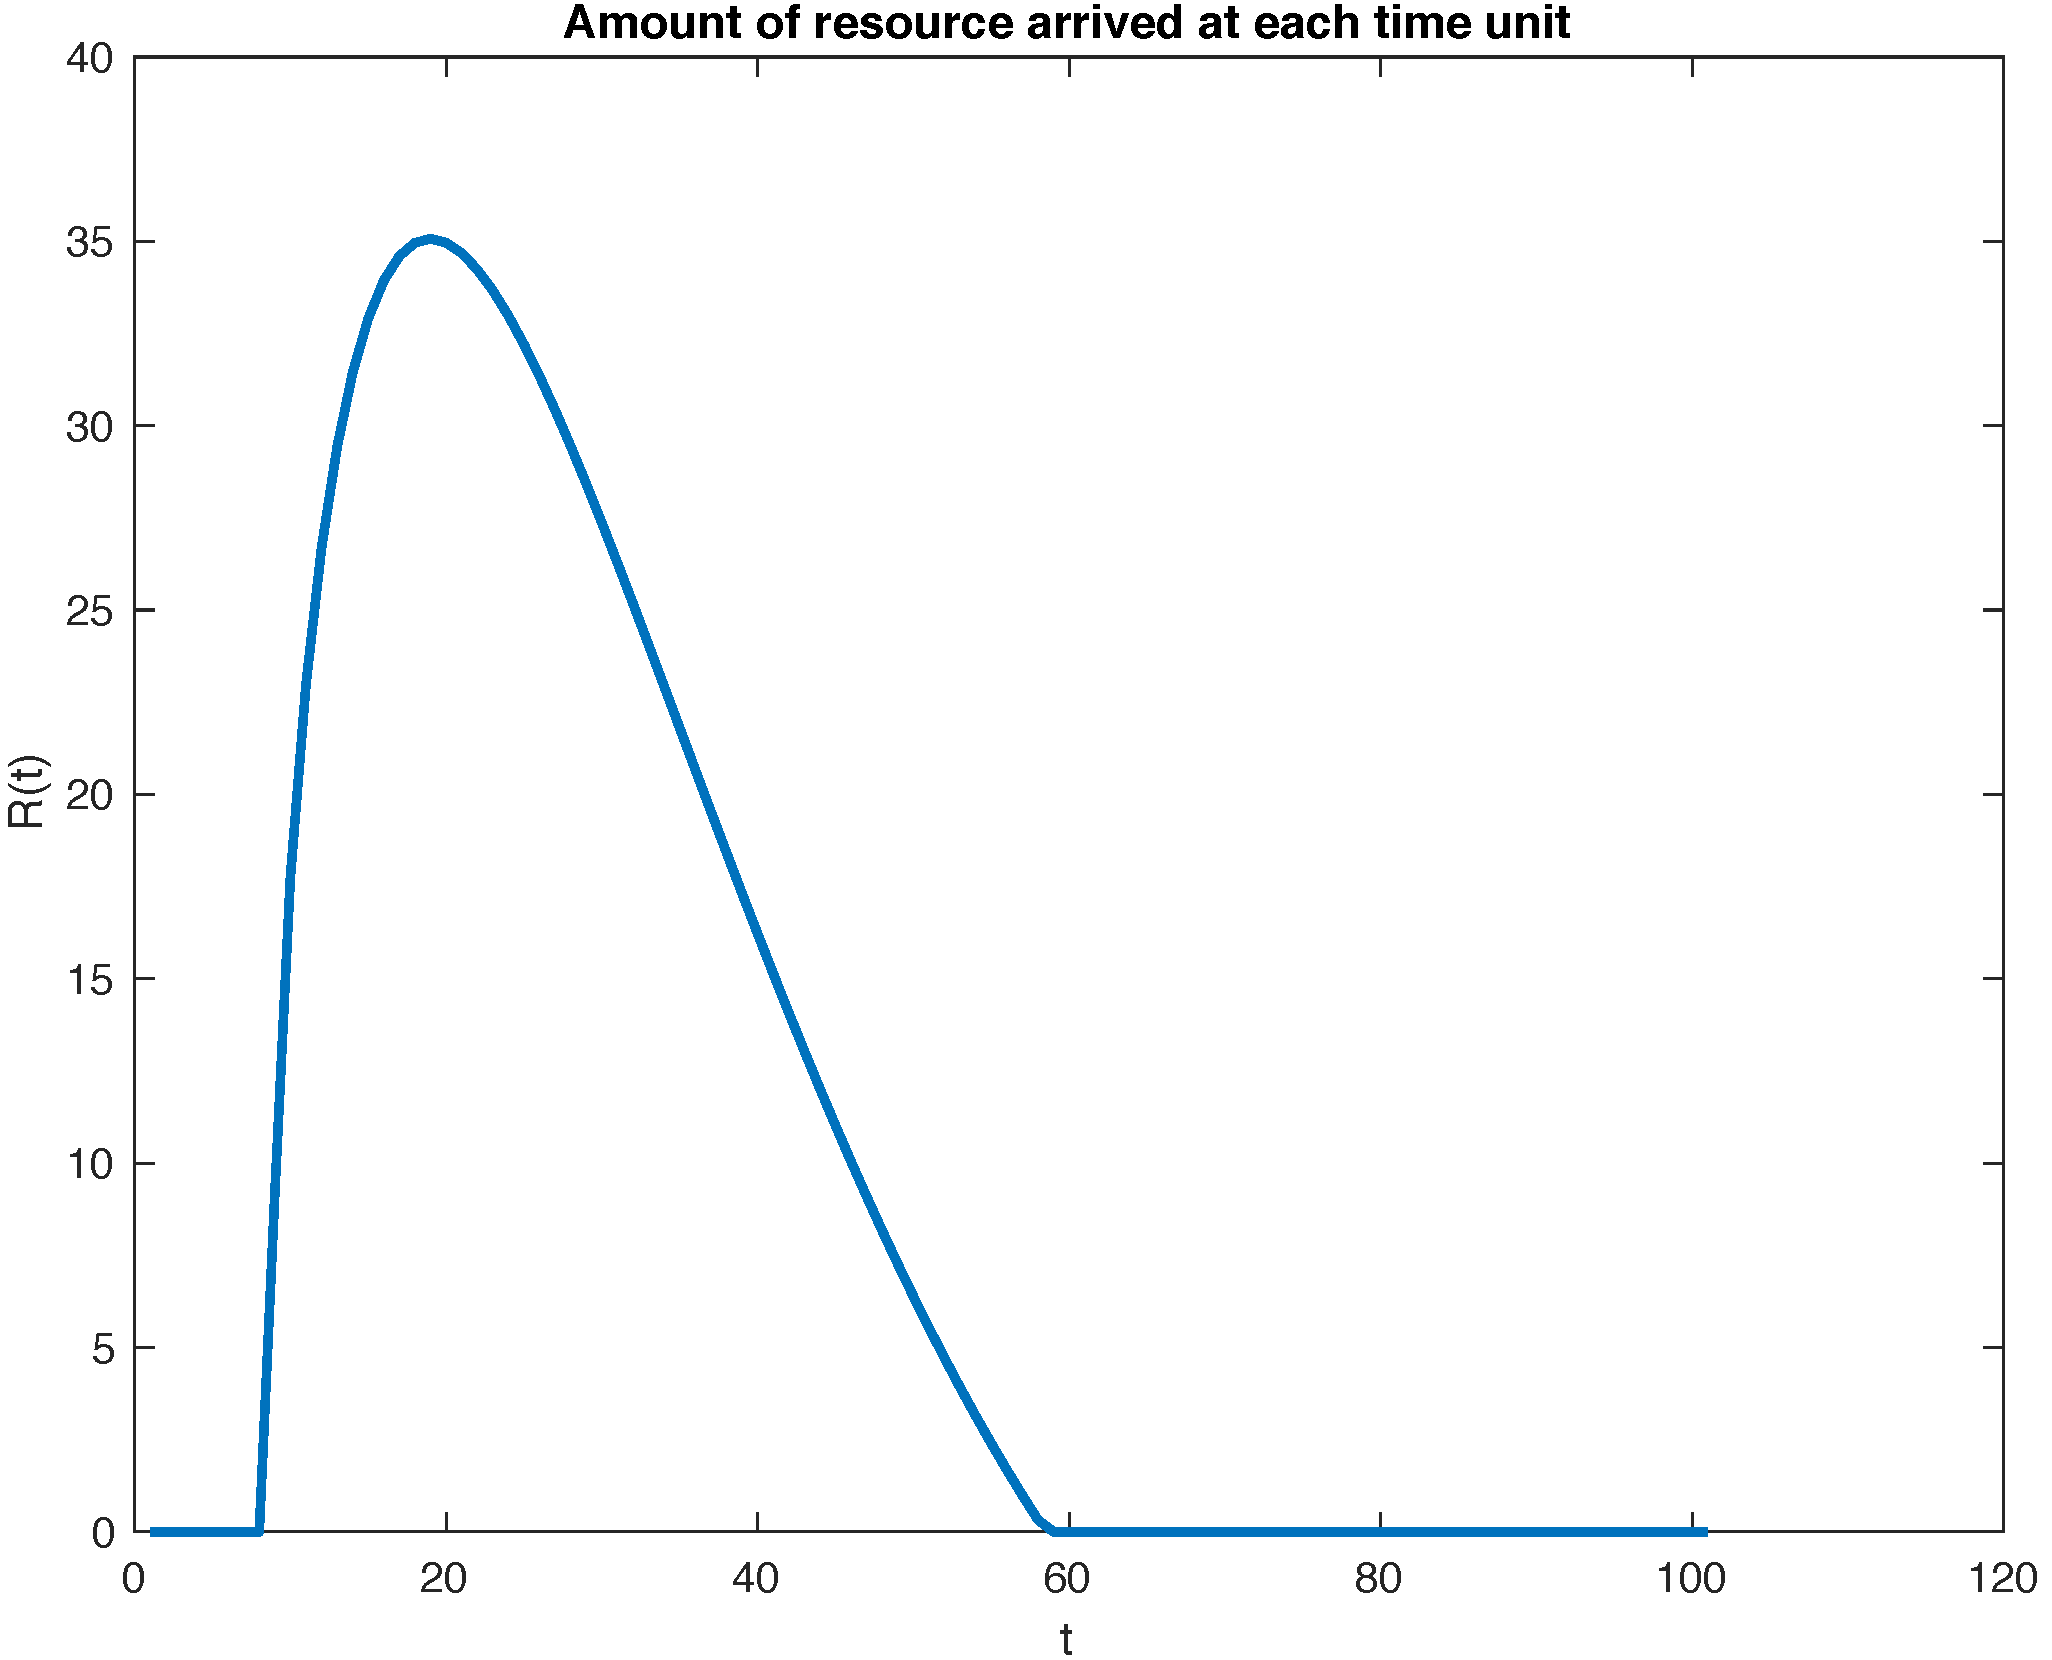
\includegraphics[height=80mm]{../figs/resource_small.pdf}
	\caption{Resource arriving at each time unit. $t_D=8$ and total resource is set to 1000.}
	\label{fig:resource}
\end{figure}

\subsection{Experiments setup}
\label{sec:experimentsSetup}
In this report, we first benchmarked our code with results in \cite{buzna2007efficient}. Then we studied effects of the choice of sigmoid coupling function in spreading model (Eq. (\ref{eq:sigmoid}) ) and replaced it with a linear function. Results showed that these two setups will lead to very different behaviors of the process. A sigmoid function with a large $\alpha$ prompts an easier spreading of disaster. 

After reproducing the results of original paper, we evaluate our optimization model. We choose two different objective functions (the first term in Eq. (\ref{eq:Lagrange}) ):  $\frac{1}{n}\sum_{i=1}^n x^{(i)}_T$ and $\sum_{i=1}^n \Theta(x_T^{(i)})$.  $\Theta(\cdot)$ is the same sigmoidal function as defined in Eq. (\ref{eq:sigmoid}). The first choice comes from that we want to minimize the averaging damage level of all nodes, while the second choice will lead to a minimization of total number of damaged nodes at time $T$. Detailed comparison of these two setups will be in Section \ref{sec:results}.

\section{Simulation Results and Discussion}
\label{sec:results}
For the numerical experiments, we firstly run the same experiments of \cite{buzna2007efficient} anc reproduce \emph{figure 2} in original paper\cite{buzna2007efficient}. Then we compare the strategy derivated by our optimization with these six heuristic strategies.

\subsection{Reproducing Experiments of Original Paper}

In order to prove the correctness of our model and codes, we firstly run the same experiments in original paper\cite{buzna2007efficient} and reproduce the \emph{figure 2} in \cite{buzna2007efficient}.


\begin{figure}	
	\centering
	\begin{subfigure}[t]{0.8\textwidth}
		\centering
		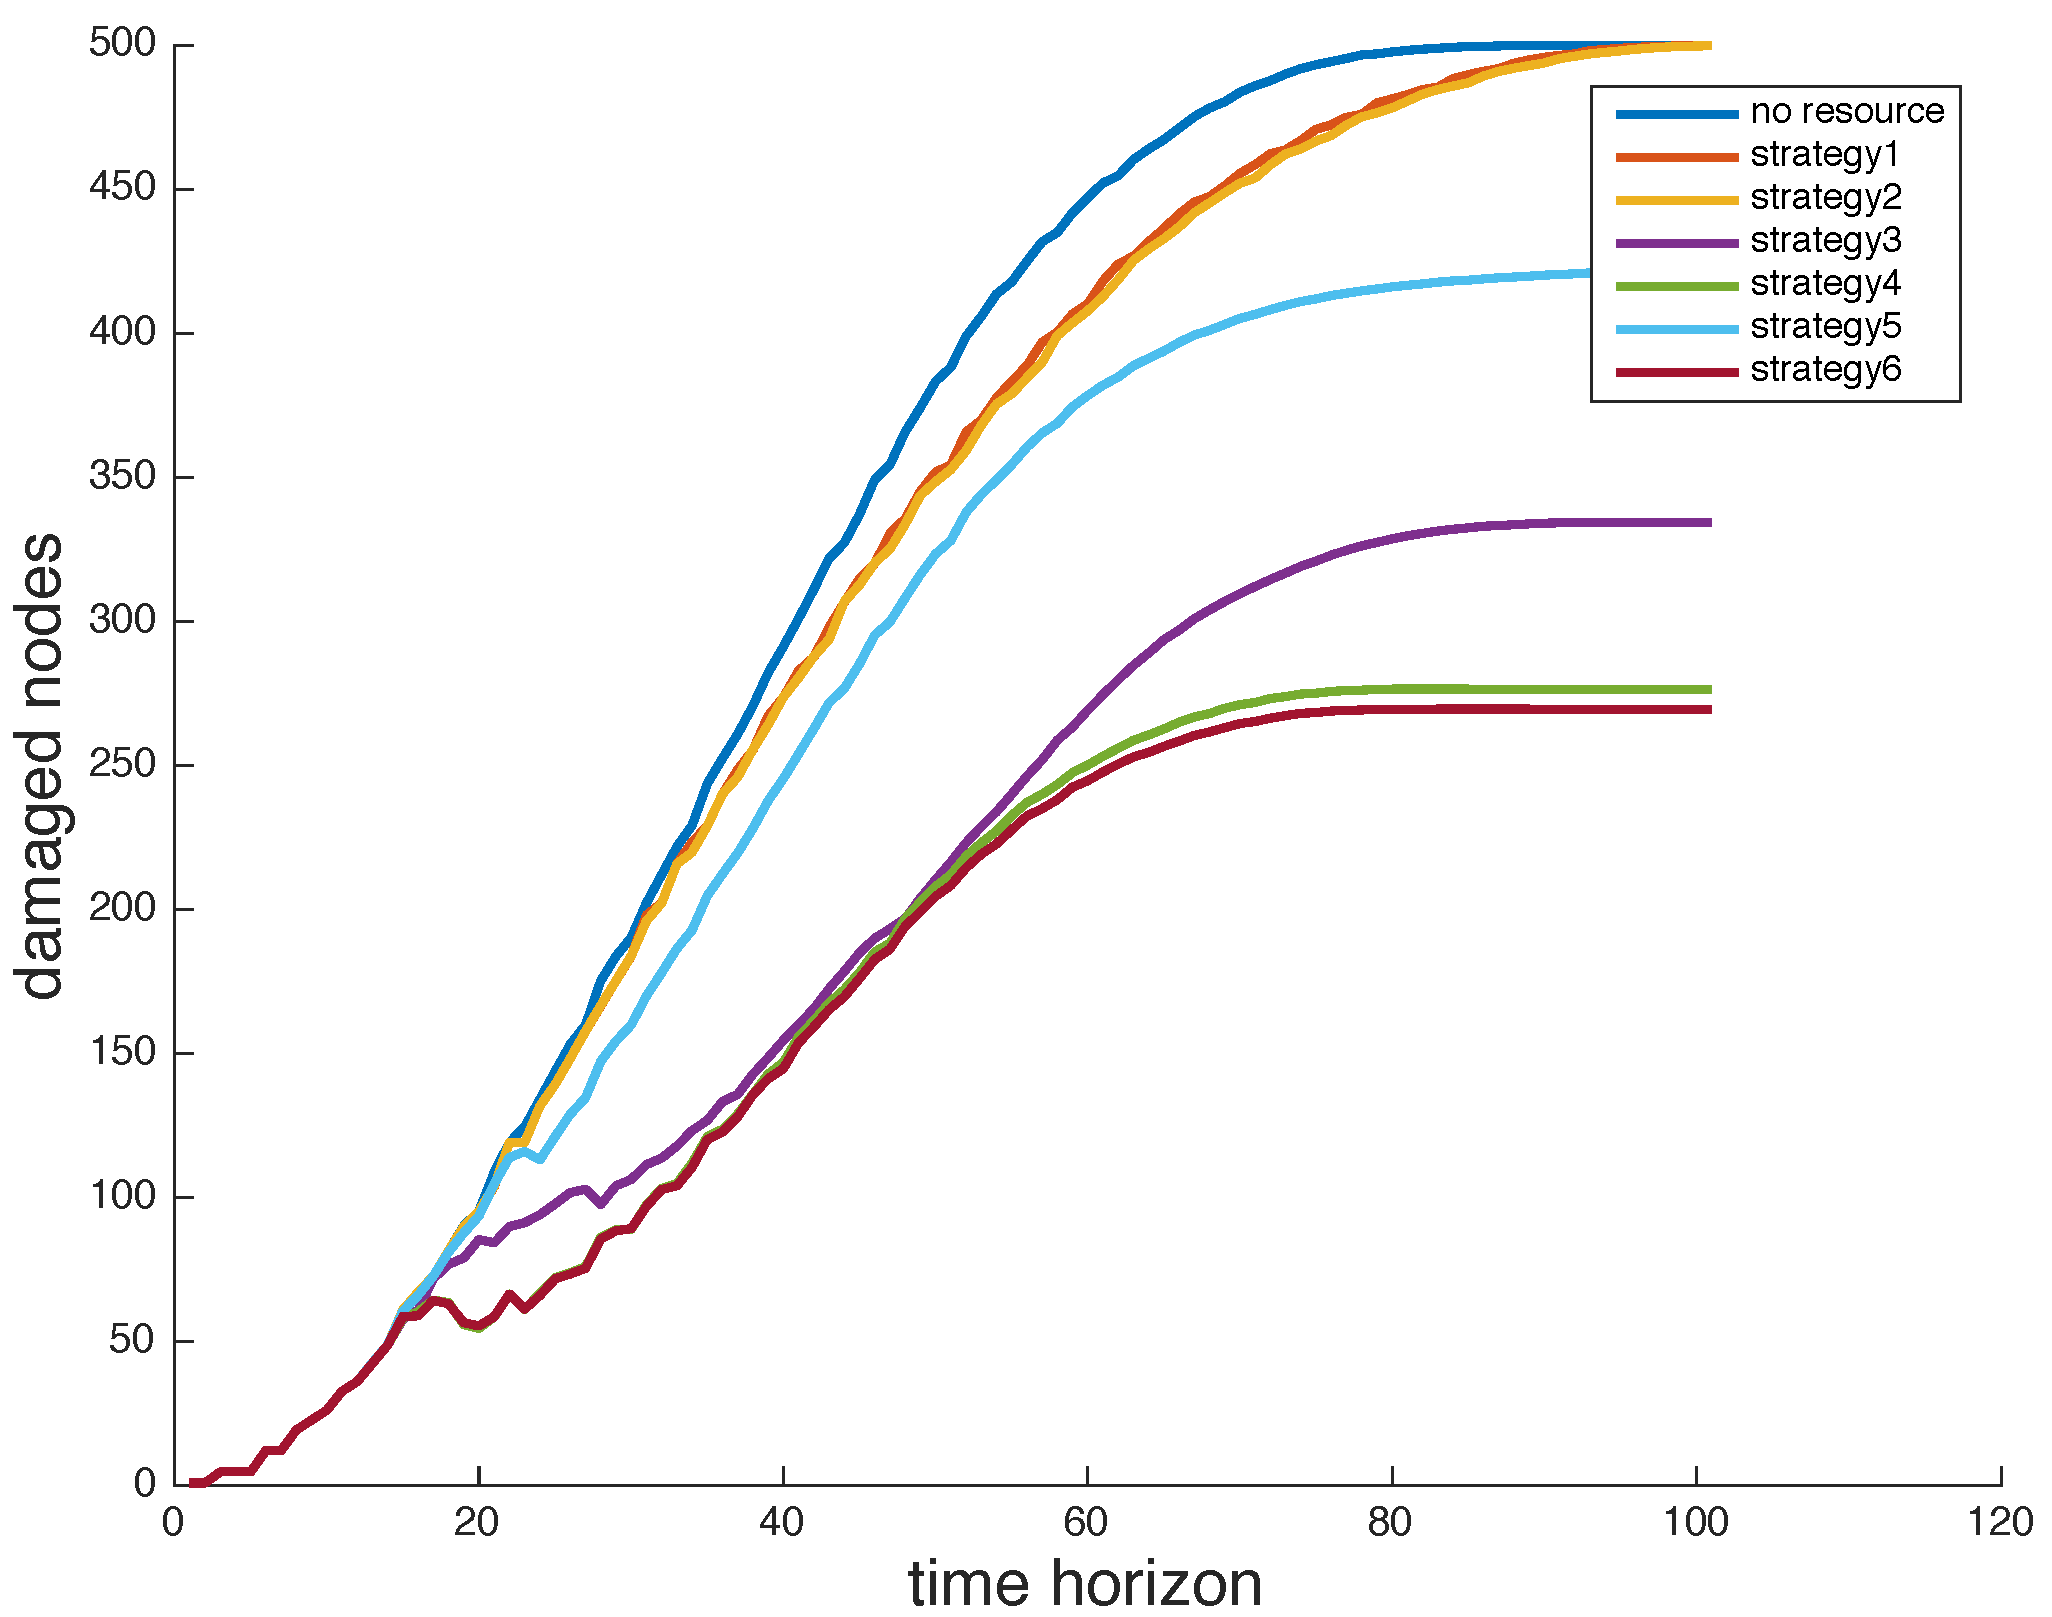
\includegraphics[height=80mm]{../figs/GridNet_original_paper2.pdf}
		\caption{Heuristic strategies on GRID network}
	\end{subfigure}
	~
	\begin{subfigure}[t]{0.8\textwidth}
		\centering
		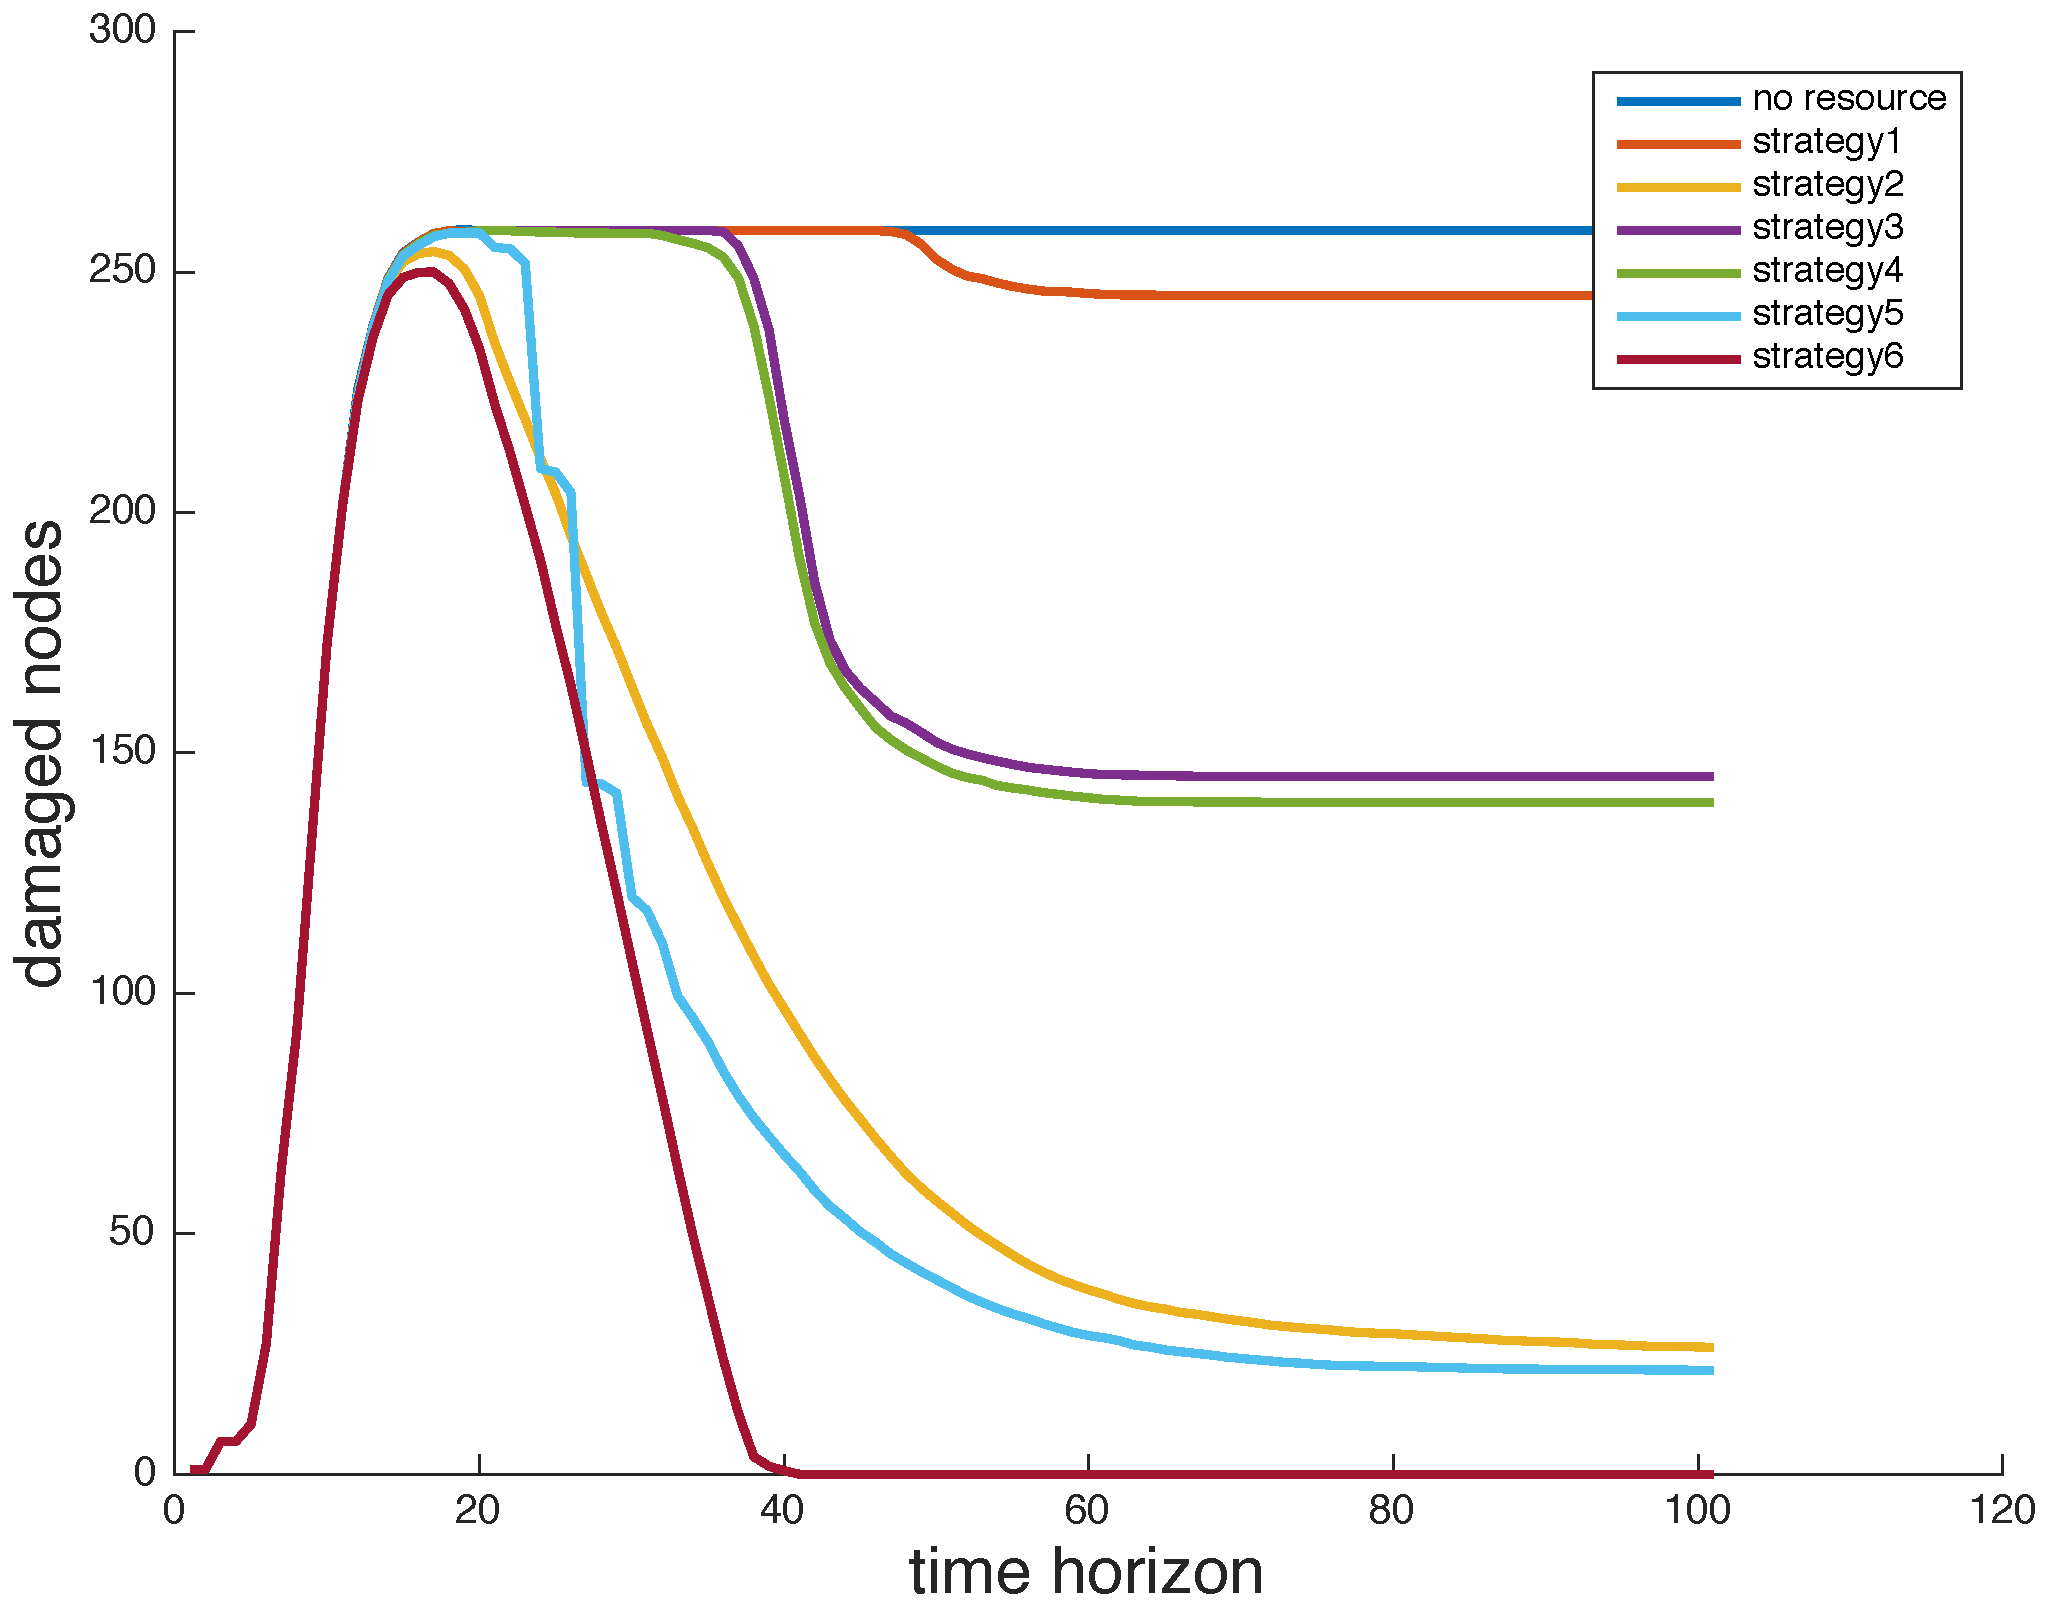
\includegraphics[height=80mm]{../figs/SFNet_original_paper2.pdf}
		\caption{Heuristic strategies on ScaleFree network}
	\end{subfigure}
	\caption{Average number of damaged nodes in (a) grid network and (b) scale-free network, with different heuristic strategis. Total external resources is 1000 and $t_D=8$. The initial damaged node is chosen randomly and these curves is average of 50 experiments.}
	\label{fig:reproduceresult}
\end{figure}
%
we can see that our result (FIG. \ref{fig:reproduceresult}) is almost the same with that in original paper\cite{buzna2007efficient}. This proves the consistency between our model and original model. So, we can further derivate the optimal strategy.

\subsection{The Optimal Strategy}
As said before, we model the disaster spreading as an optimization problem and the solution to this optimization problem corresponds is exactly the optimal strategy to distribute external resources. We have introduced this optimization model in Sec. \ref{sec:adjointmethod} and specified its details in Appendix \ref{sec:appendix1}. Now, we compare the derivated optimal strategy with these six heuristic strategies.


\begin{figure}
	\centering
	\begin{subfigure}[t]{0.8\textwidth}
		\centering
		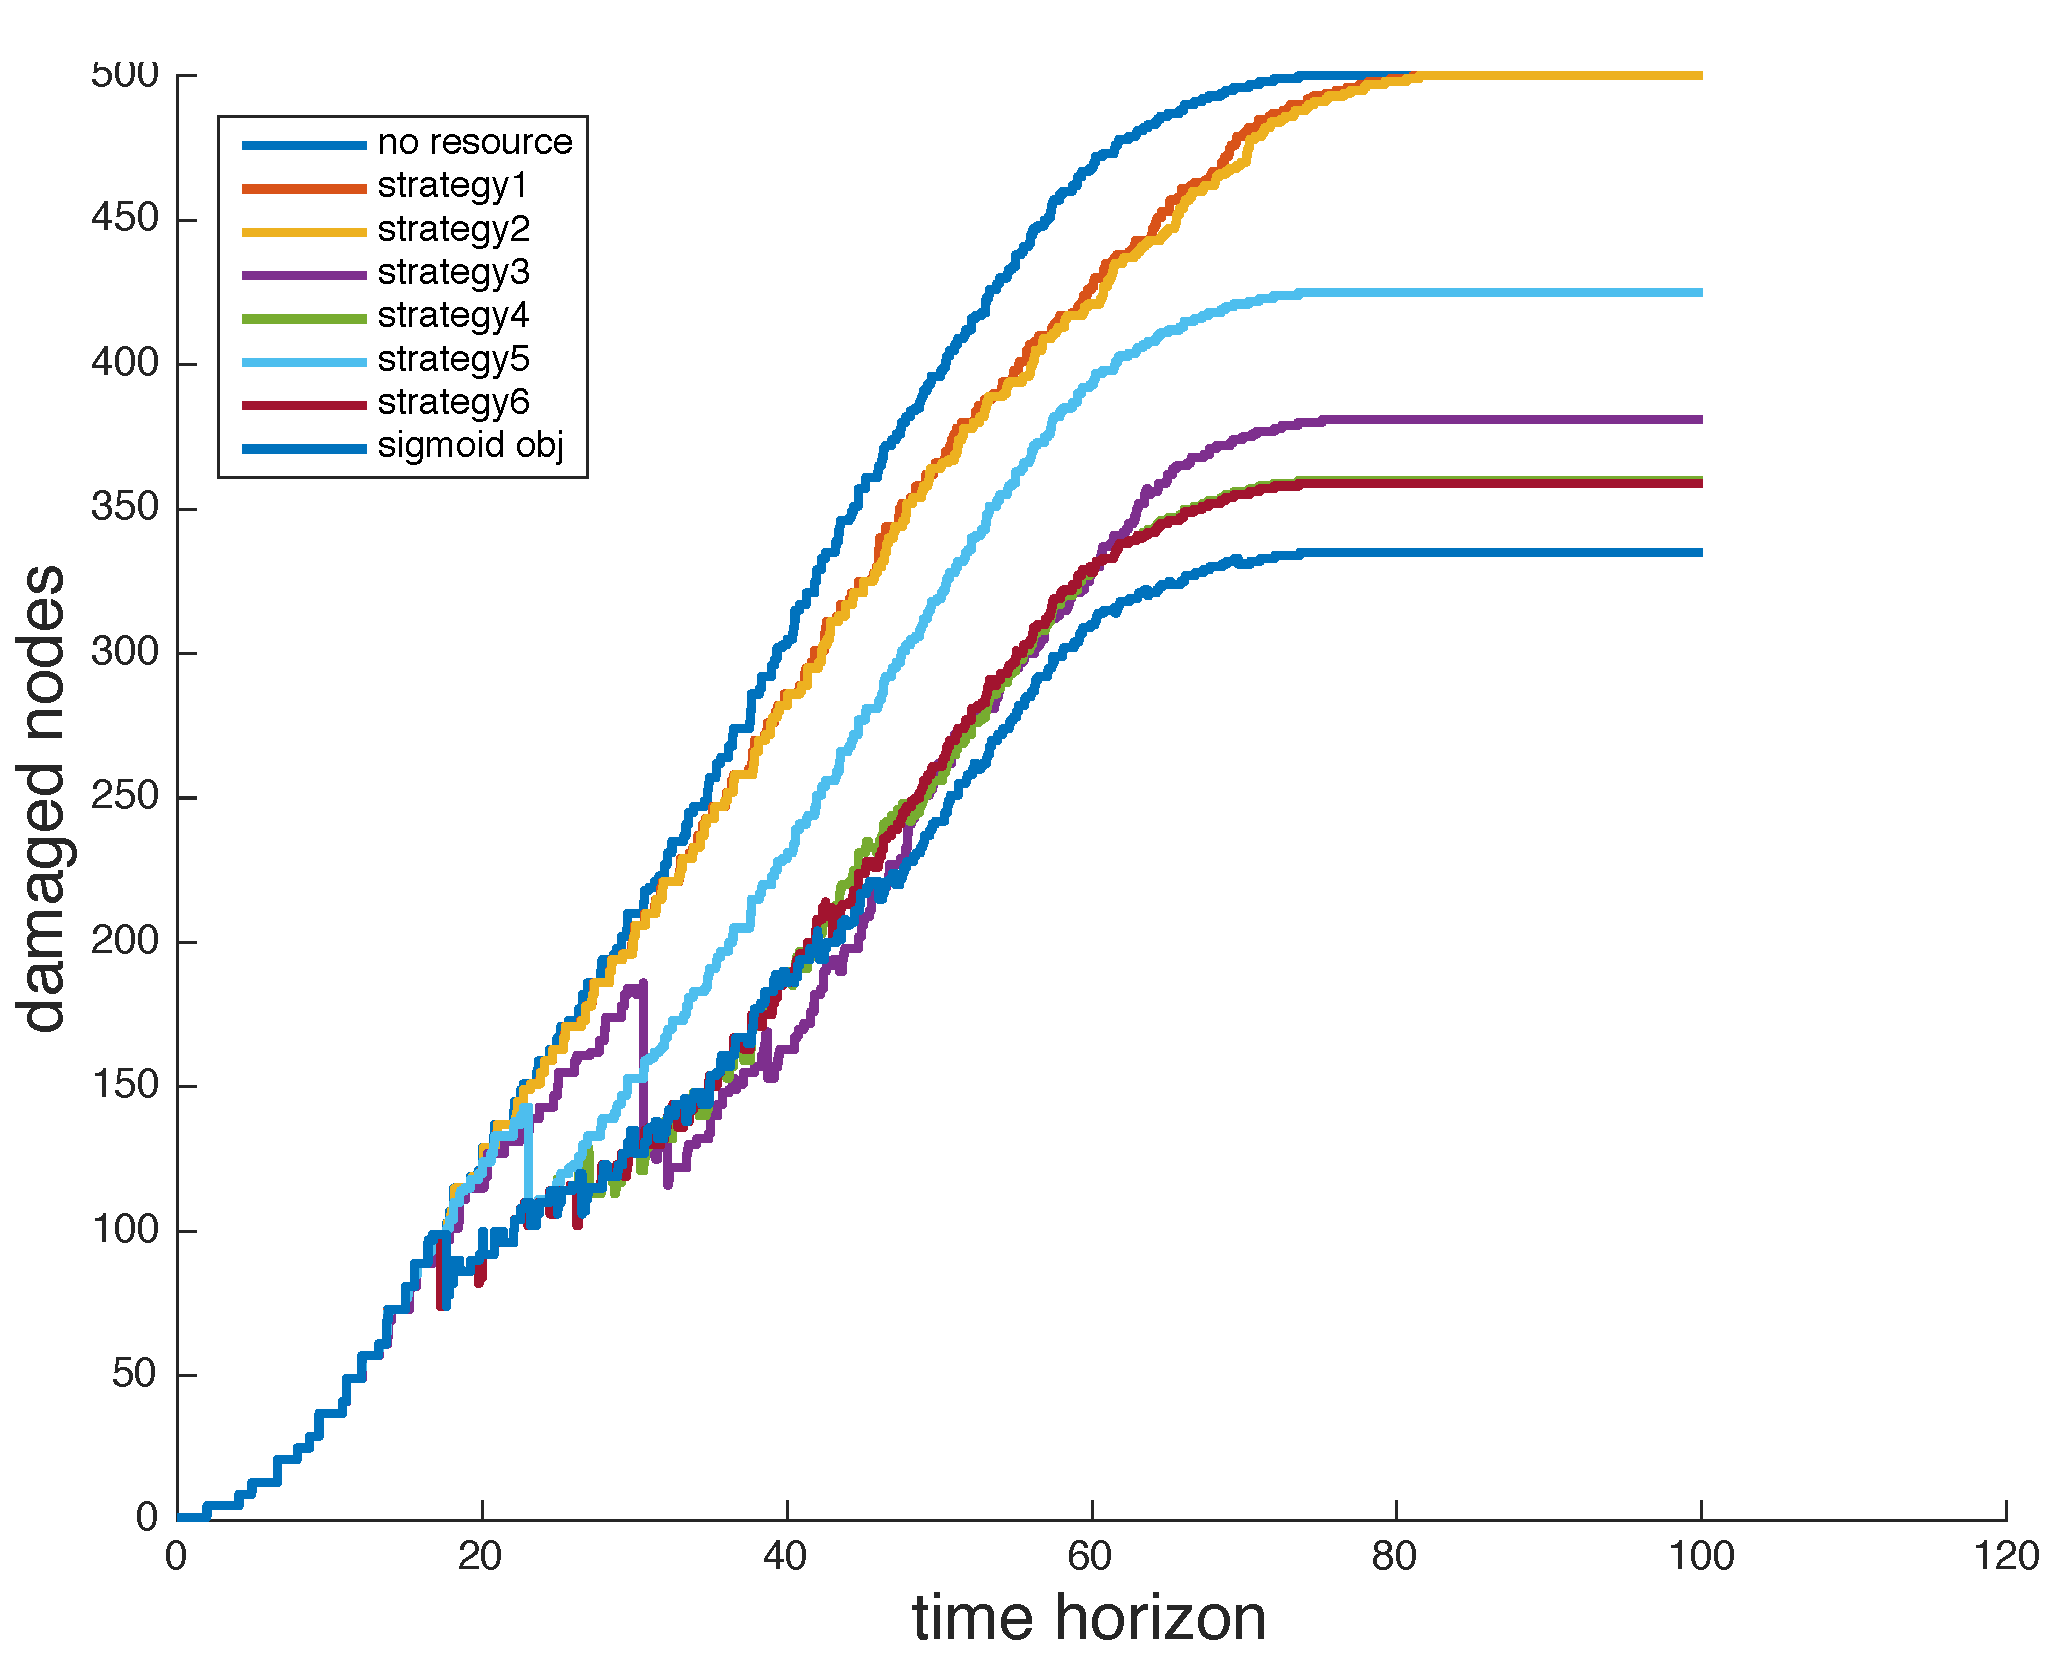
\includegraphics[height=80mm]{../figs/no_linear_approximation/Grid_damaged_small.pdf}
		\caption{Damaged nodes on grid network}
	\end{subfigure}
	~
	\begin{subfigure}[t]{0.8\textwidth}
		\centering
		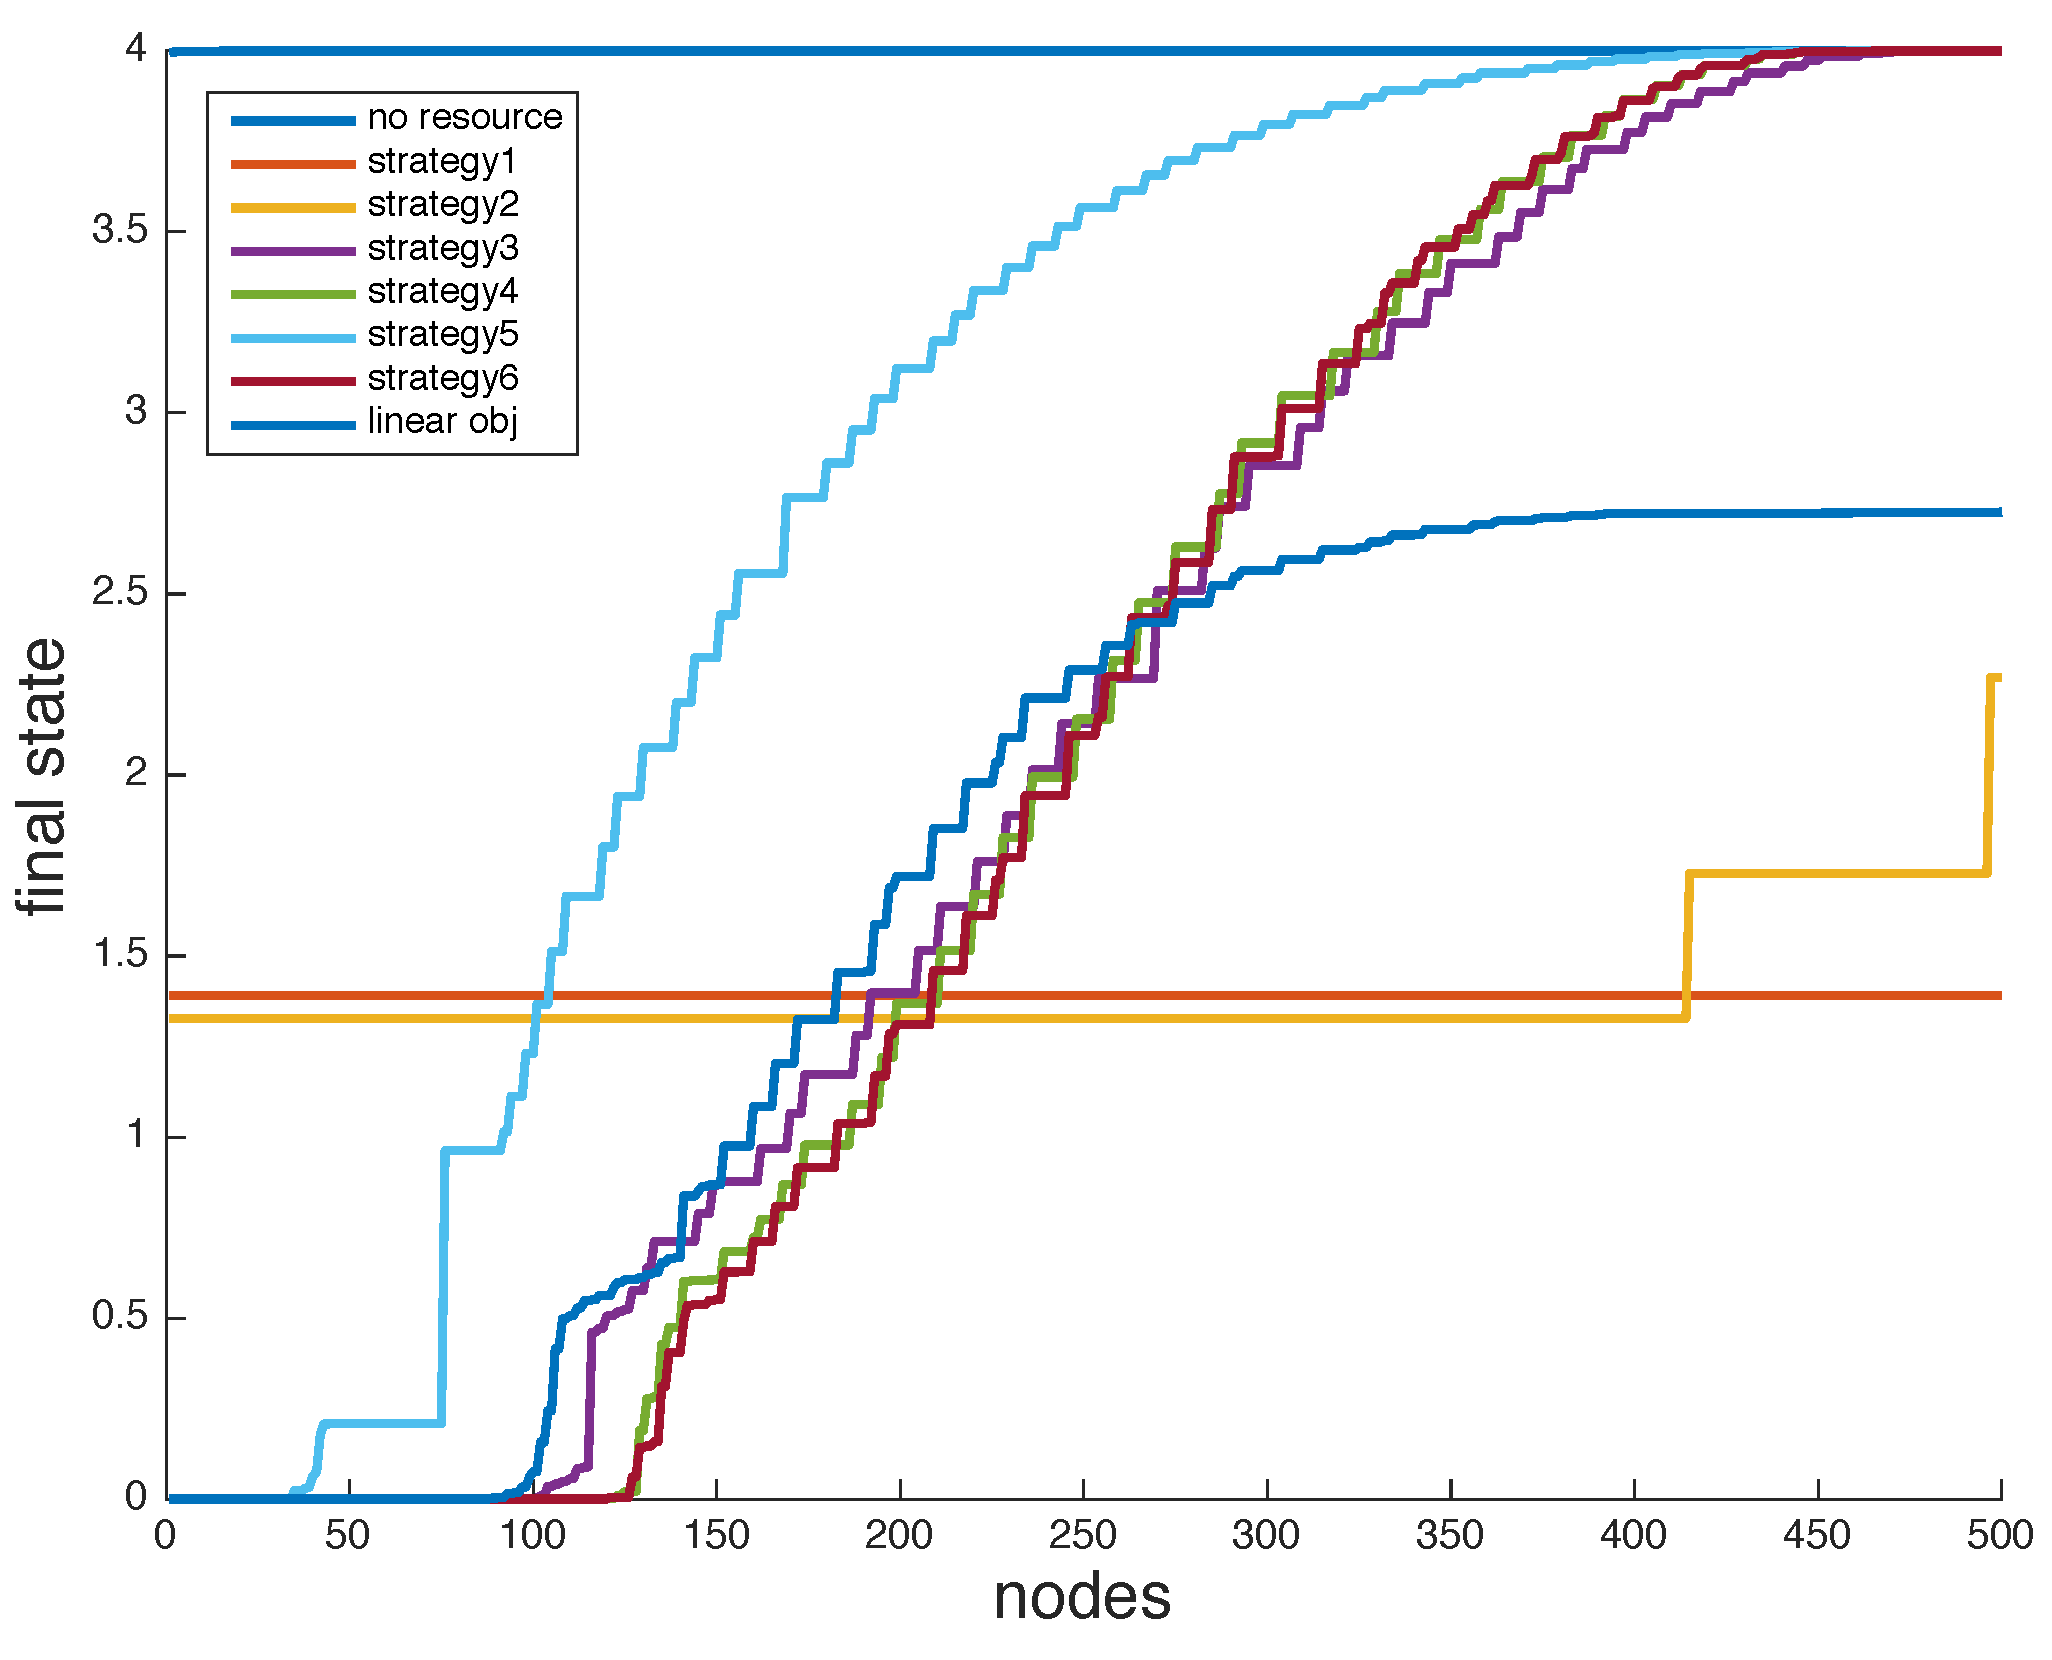
\includegraphics[height=80mm]{../figs/no_linear_approximation/Grid_finalState_small.pdf}
		\caption{Final states on grid network}
	\end{subfigure}
	\caption{(a) Number of damaged nodes and (b) final states on grid network. Total external resources is 1000 and $t_D=8$. The initial damaged node is chosen randomly. The maximal iterations of gradient descent is 100.}
	\label{fig:opt_on_grid}
\end{figure}

We first minimize the number of damaged nodes. A natural objective function for this purpose is 0-1 loss function:

\begin{equation}
	\label{eq:0_1_loss}
	\begin{aligned}
		J &= \sum_i h(x_i) \\
		\text{where } h(\cdot) &= 
		\begin{cases}
			1 & \text{if } x_i \ge \theta_i \\
			0 & \text{otherwise}
		\end{cases}
	\end{aligned}
\end{equation}

However, this objective function is not continuous and cannot be optimized by the adjoint method. So we use again the sigmoid function to approximate this 0-1 loss function:

\begin{equation}	
	\label{eq:sigmoid2}
	\Theta_i(y) = \frac{1-\exp(-\alpha y)}{1+\exp(-\alpha (y-\theta_i))}
\end{equation}

The $\alpha$ parameter in formula \ref{eq:sigmoid2} controls its shape. We find that the sigmoid can approximate the 0-1 loss function very well with $\alpha \leq 20$. So we set $\alpha=20$ and compare the derivated strategy with other six heuristic strategies. Fig. \ref{fig:opt_on_grid} shows that this derivated optimal strategy do decrease the number of damaged nodes.

\begin{figure}
	\label{eq:sigmoid_alpba}
	\centering
	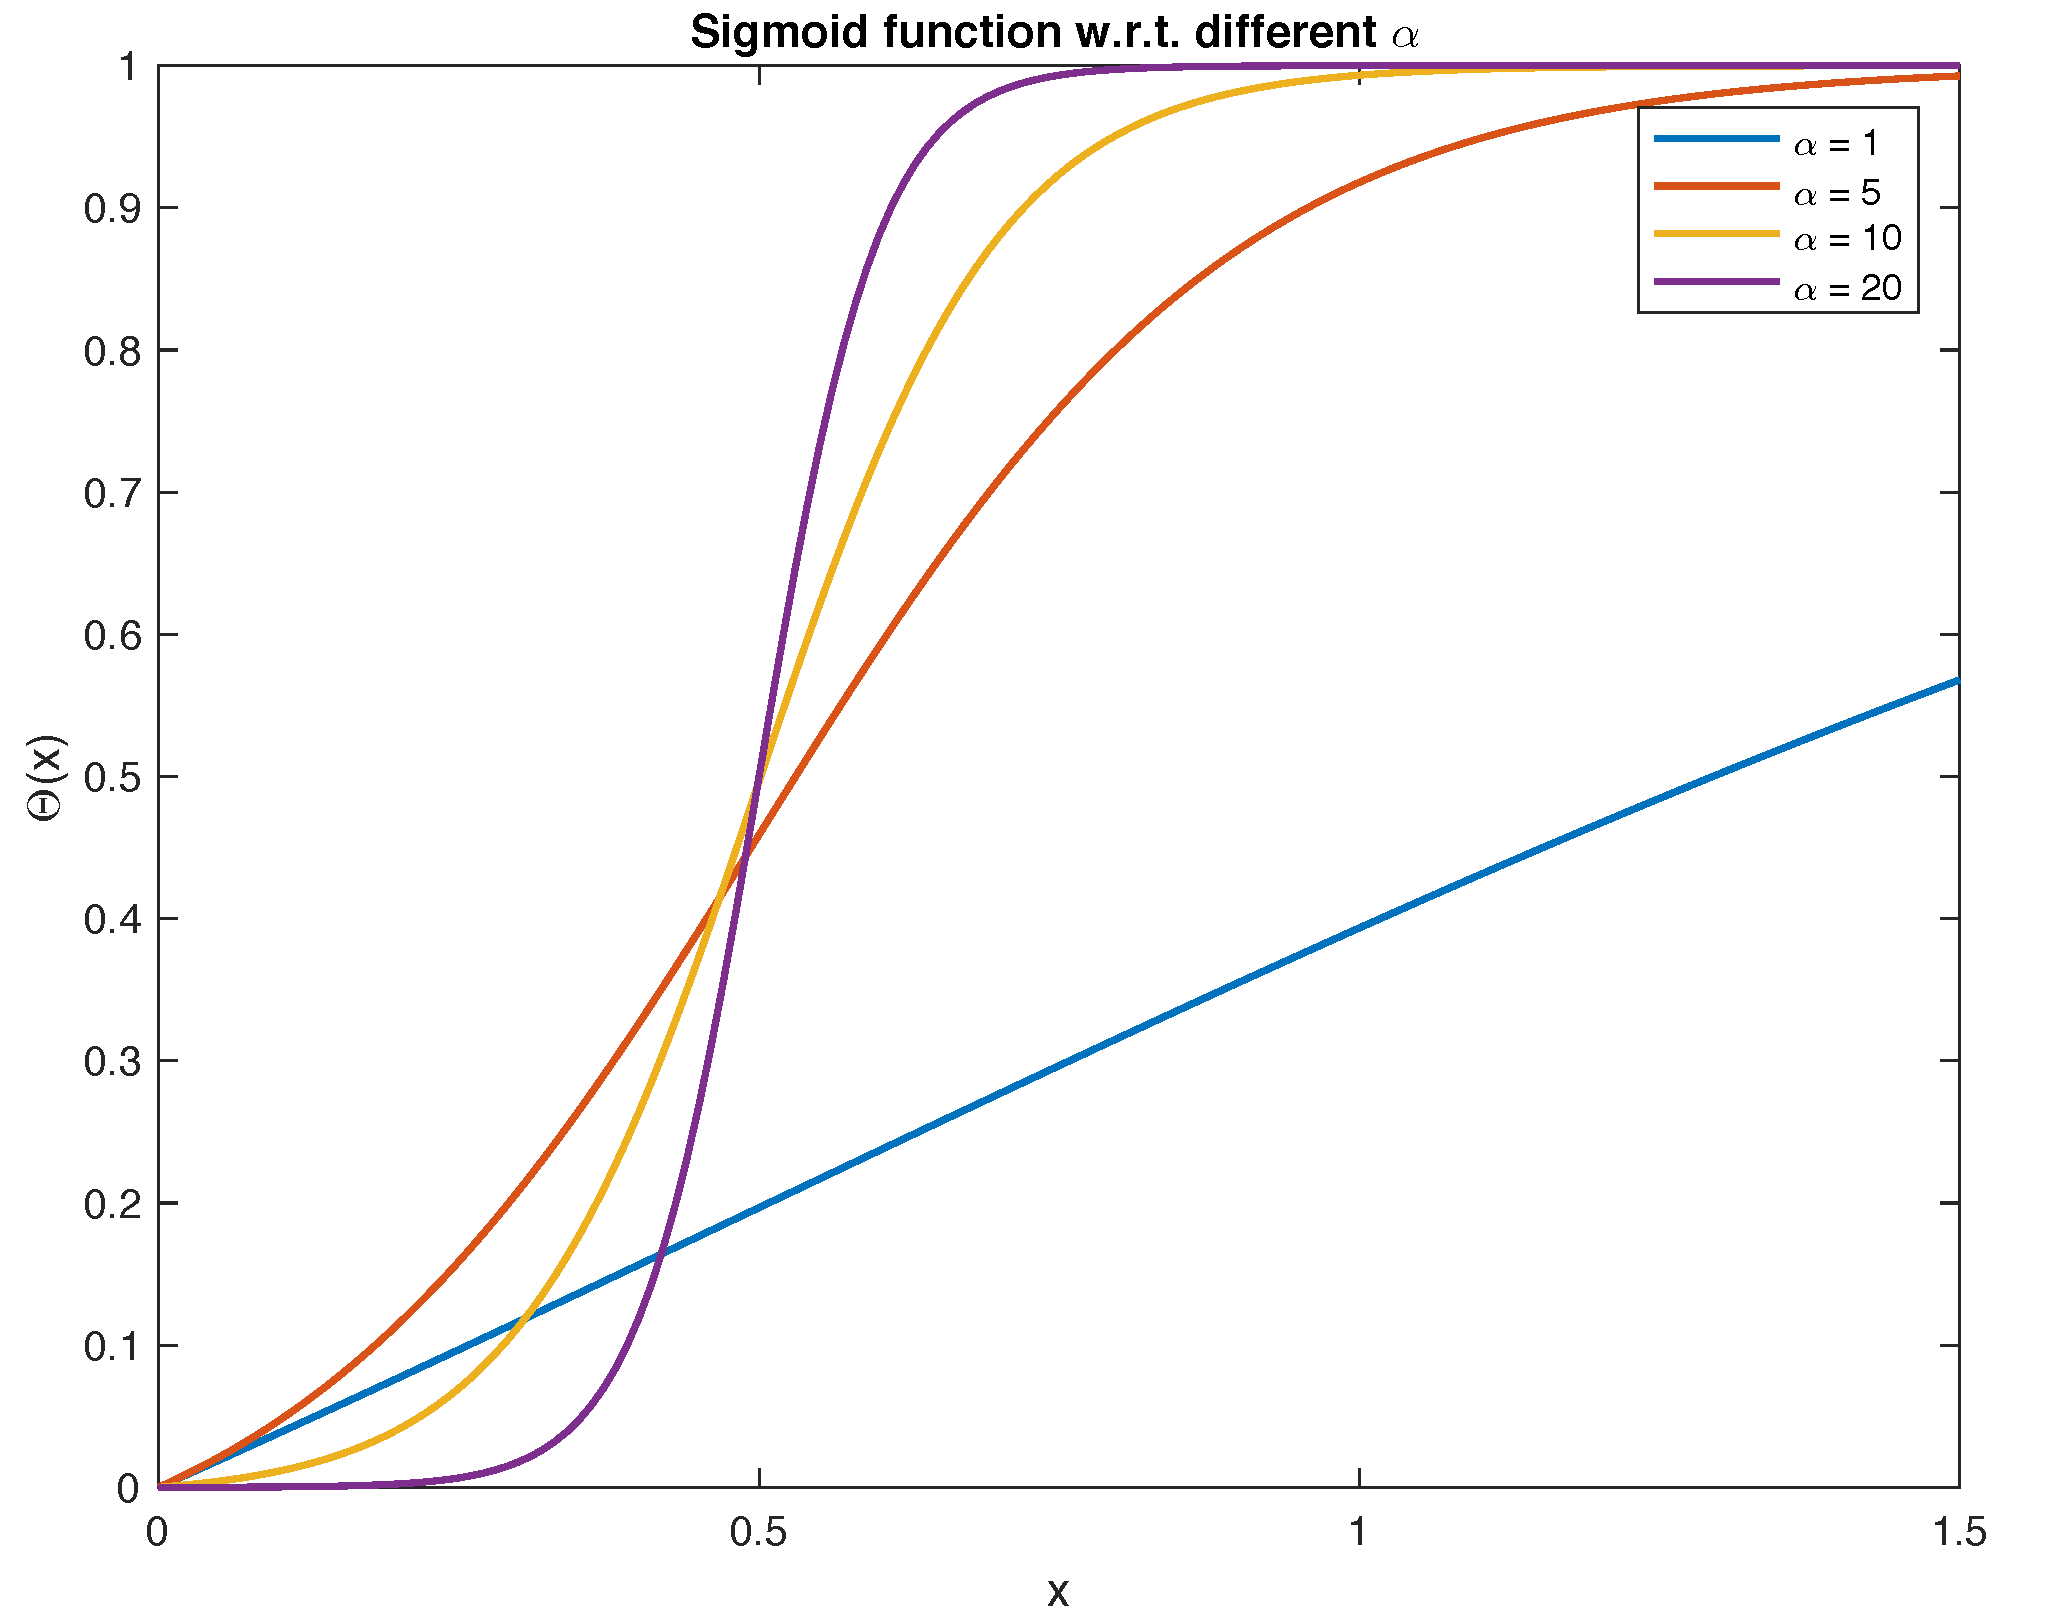
\includegraphics[height=60mm]{../figs/sigmoid_small.pdf}
\end{figure}

However in some cases, we care about the states of all nodes and we do not want to lose control on some nodes. And it is not insufficient to use the number of damaged nodes as criterion to evaluate strategies, since some strategy may abandon those nodes which are severely damaged. Based on such consideration, we proposed the other objective function:

\begin{equation}
\label{eq:obj2}
	J = \frac{1}{n} \sum_i x_i
\end{equation}

Eq. \ref{eq:obj2} aims at optimizing the average state of all nodes. It exclude the situation that some nodes are out of control. FIG. \ref{fig:opt_on_grid} (b) compares the optimal strategy corresponding to this objective function with other heuristic strategies. We can find that the derivated optimal strategy do optimize the states of all nodes.


Besides the grid network, we also perform the same experiments on scale-free network. The result (FIG. \ref{fig:opt_on_sf}) shows that the derivated strategy is again better than other six heuristic strategies.

\begin{figure}	
	\centering
	\begin{subfigure}[t]{0.8\textwidth}
		\centering
		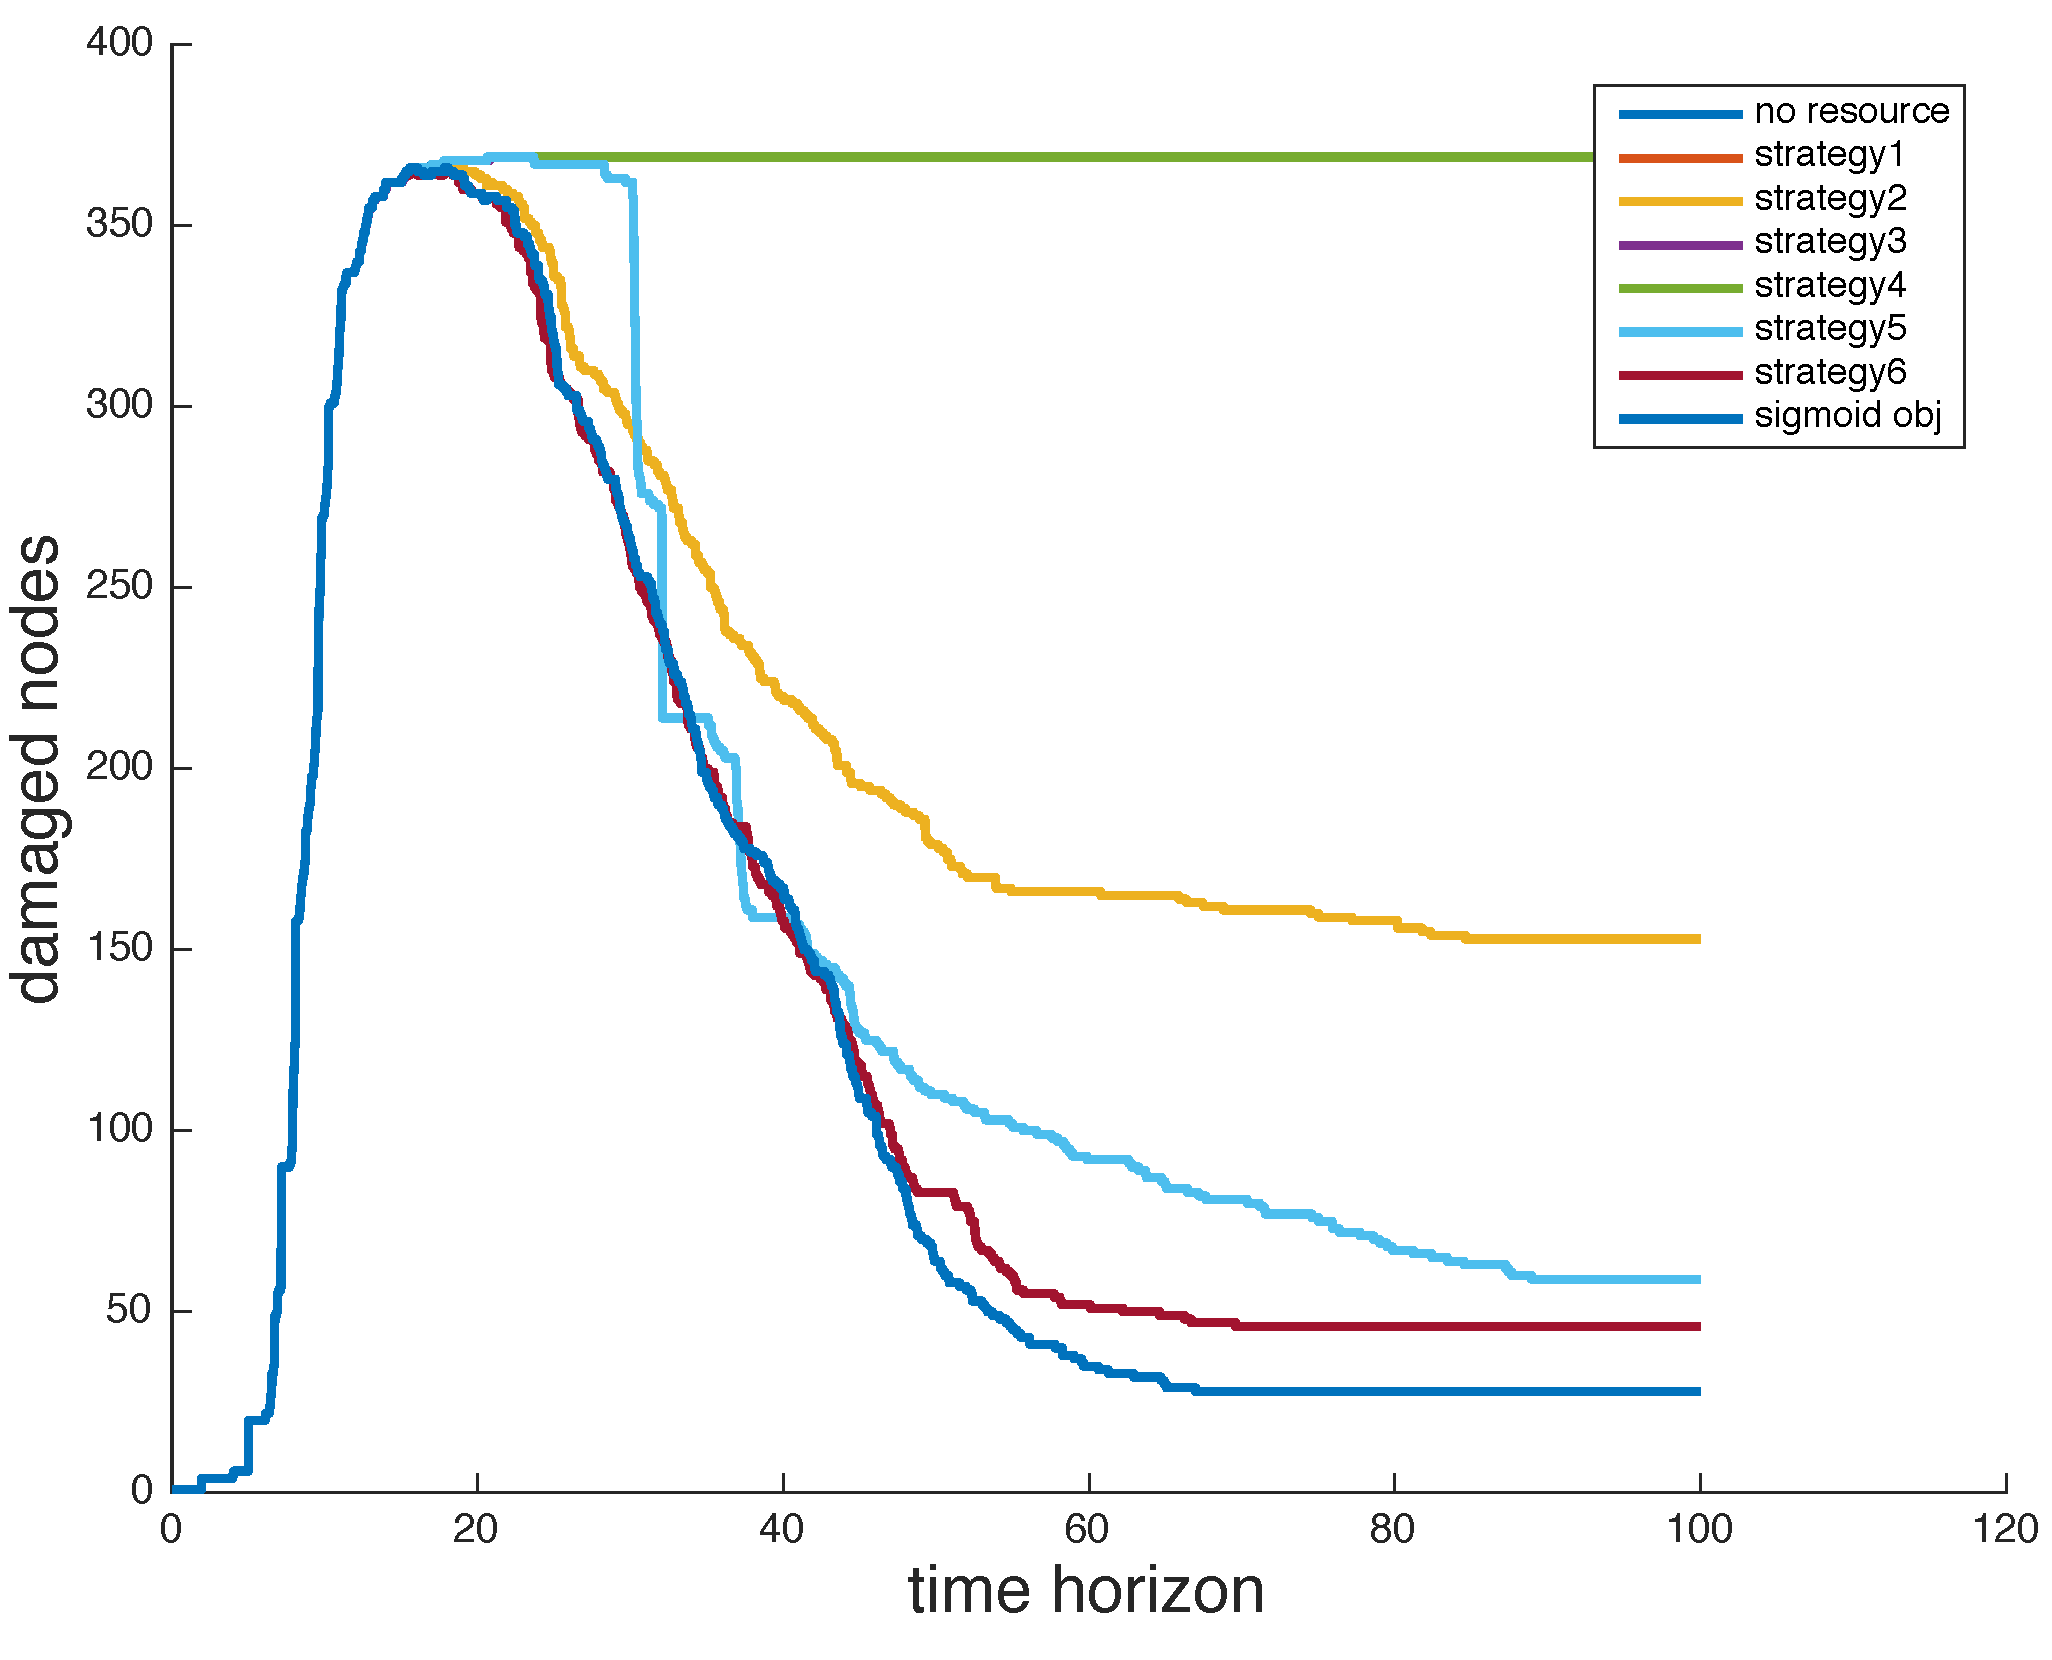
\includegraphics[height=80mm]{../figs/no_linear_approximation/SF_damaged_small.pdf}
		\caption{Damaged nodes on scale-free network}
	\end{subfigure}
	~
	\begin{subfigure}[t]{0.8\textwidth}
		\centering
		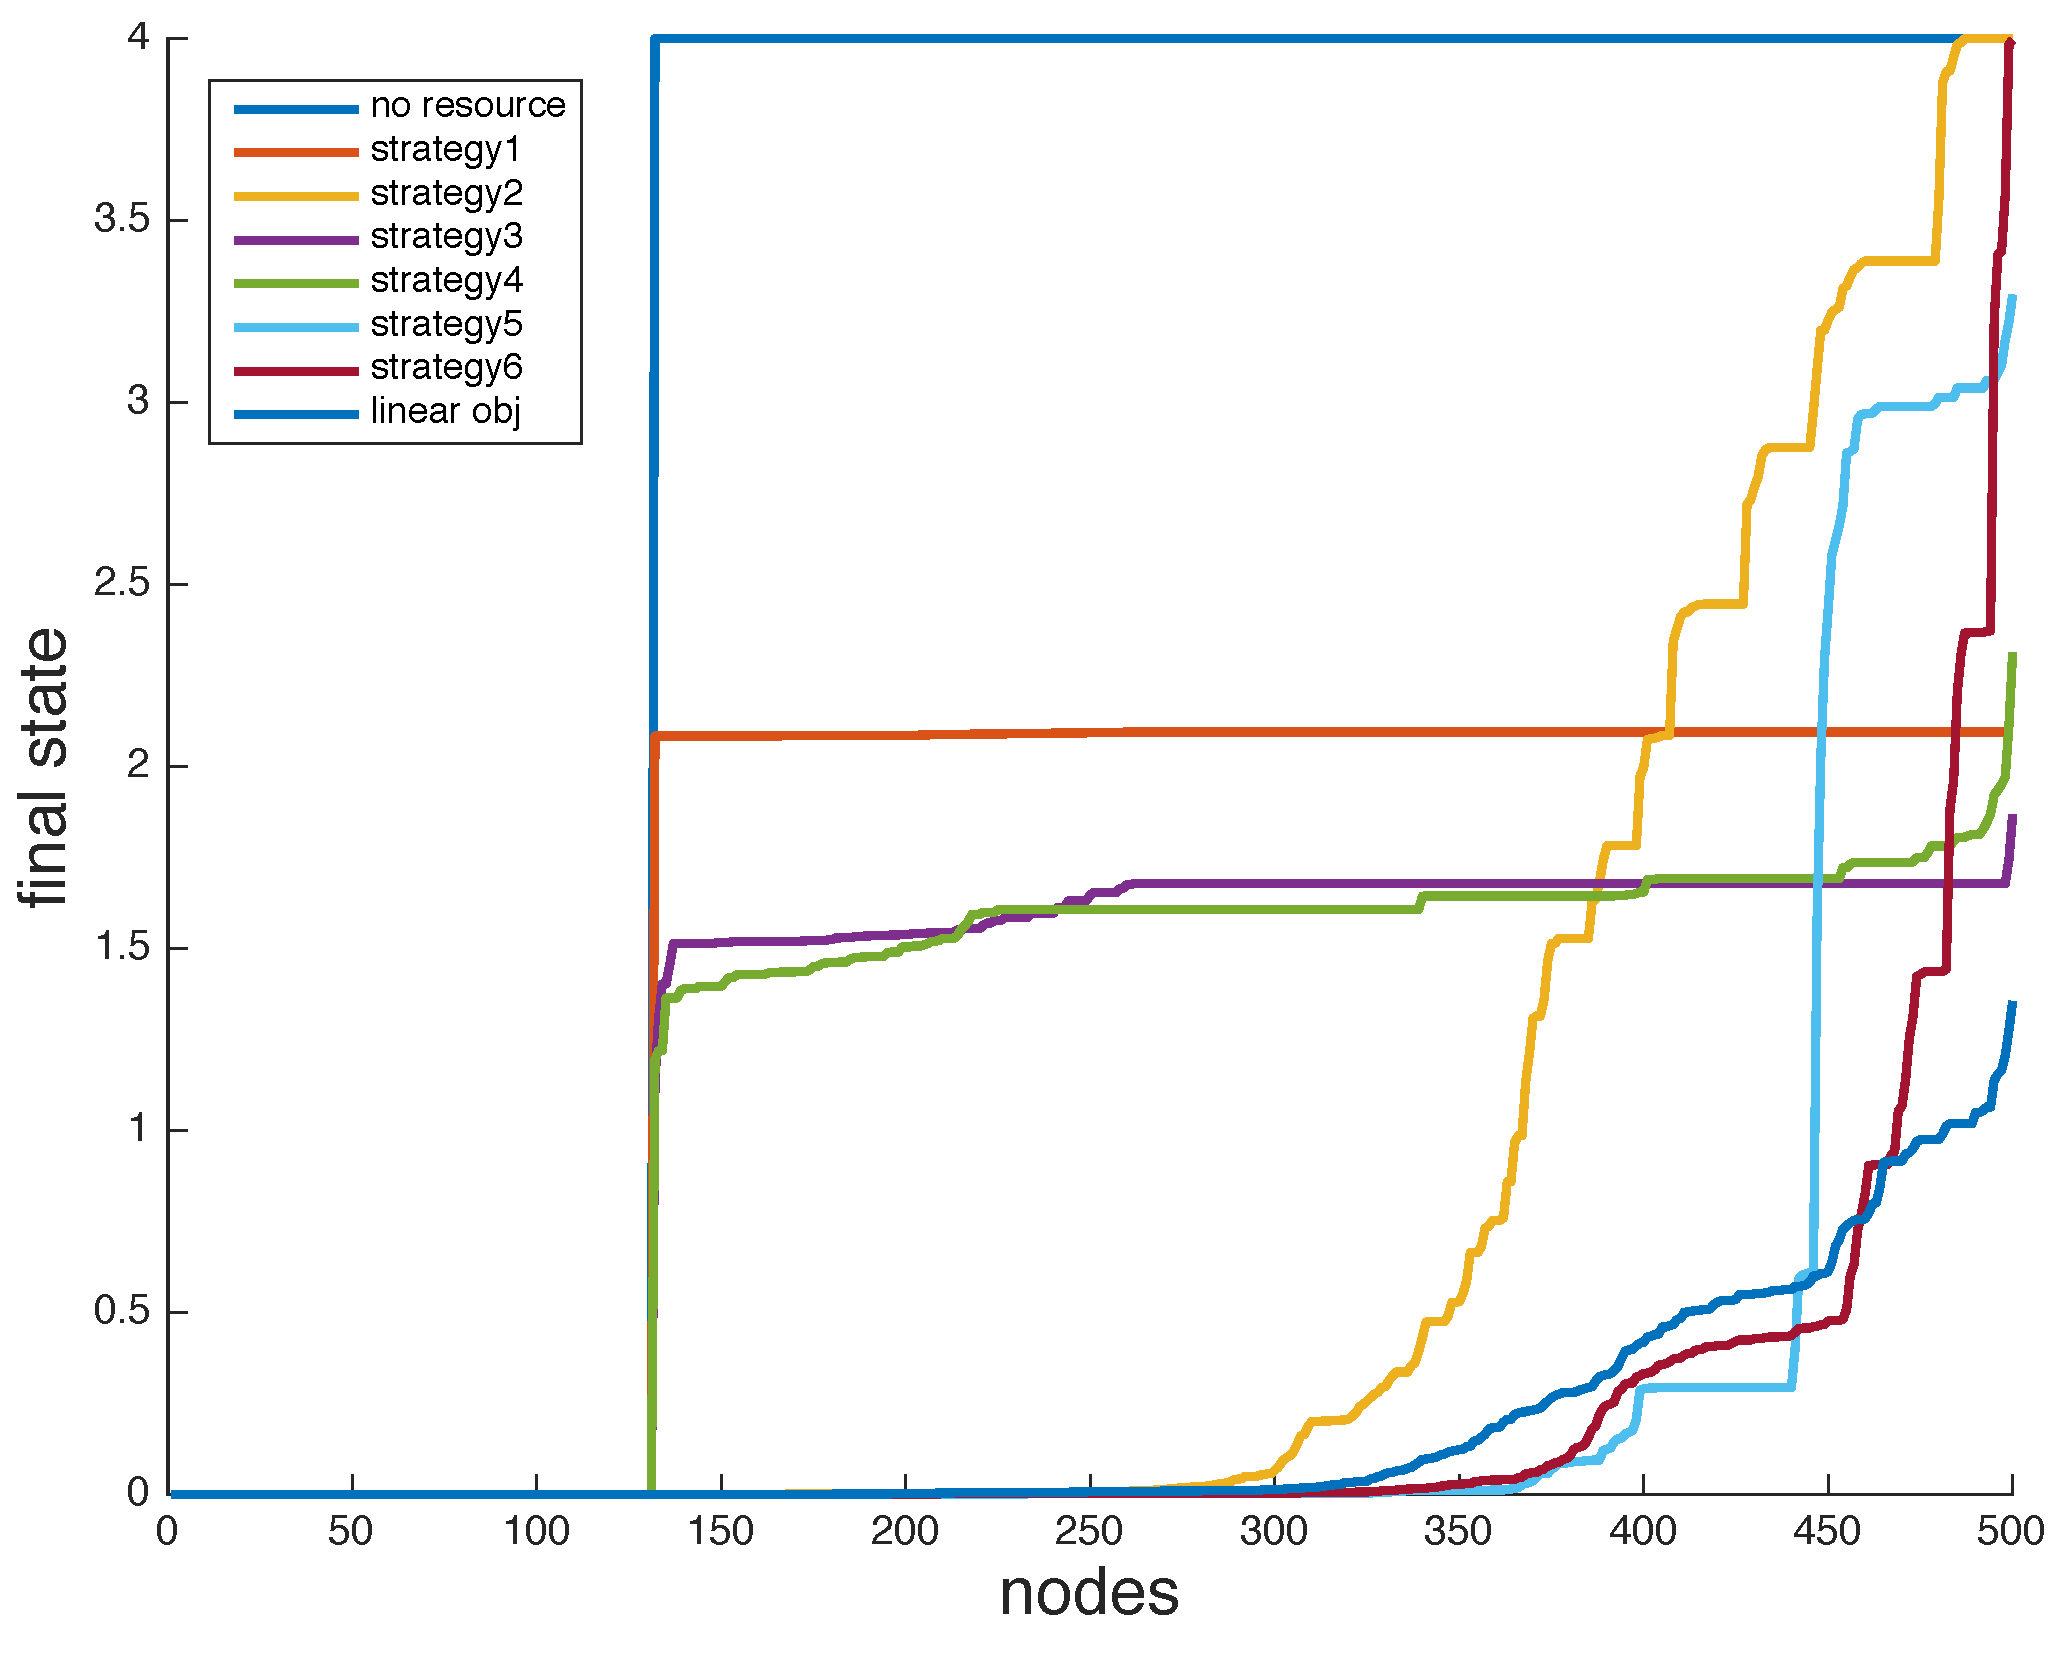
\includegraphics[height=80mm]{../figs/no_linear_approximation/SF_finalState_small.pdf}
		\caption{Final states on scale-free network}
	\end{subfigure}
	\caption{(a) Number of damaged nodes and (b) final states on grid network. Parameter setting is the same with that in grid network except for total external resources, i.e. $t_D=8$ and maximal iterations of gradient descent is 100. Because \textbf{S6} has achieve best result with 1000 external resources, in order to discriminate these strategies we decrease external resources to 600.}
	\label{fig:opt_on_sf}
\end{figure}





\section{Summary and Outlook}
\label{sec:summary}
To sum up, we have mainly done these things in our work:
\begin{itemize}
	\item Reproduce the results in \cite{buzna2007efficient}
	\item Model disaster spreading as an PDE-constraint optimization problem and come up with two objective functions corresponding to different optimal criteria
	\item Find the optimal (may be local optimum, due to the inheritance of optimization method) strategy to distribute external resources given the network topology, by solving this optimization problem using adjoint method 
	\item Compare the optimal strategies with these six heuristic strategies on grid and scale-free networks. 
\end{itemize}

What could do further is to analyze more the optimal strategy. This may give us more understanding to control disaster.



% \section{References}
\bibliography{mybib}{}
\bibliographystyle{plain}

\section{Appendix \RN{1} -- Details about the adjoint method}
\label{sec:appendix1}
In this section we will present the adjoint system of our disaster spreading model.  For numerical implementation reason, we always need to transform the equation into a discrete version. One way to do this is to find a suitable basis to expand $r(t)$, but the choice here is not so clear in this case and we decide to discretize the resource strategy. $R_i(t)$ will be piecewise constant function, i.e. resource will only arrive at certain time, rather than a continuous function. Let us rewrite the controlling equation as 
\beq
	\frac {\pa\xx} {\pa t} = -{\ms P(t)}\xx + {\ms K}\xx, 
\eeq
in which ${\ms P(t)}$ is a diagonal matrix
\beq
	{\ms P}_{ij}(k) = \frac 1 {\tau_i(k)} \delta_{ij} = \frac{1}{(\tau_{start} - \beta_2)e^{-\alpha_2\sum_{nt = 1}^{k}\Delta R_i(nt)} + \beta_2}\delta_{ij}
\eeq
 and ${\ms K}$ is also a matrix with each element of ${\ms K}$ as a kernel function,
\beq
	{\ms K}_{ij}(t, s) = \frac{M_{ji}e^{-\beta t_{ji}}}{f(O_j)} \delta(s-t+t_{ji}), 
\eeq
 correspond to the two terms on the r.h.s of Eq. (\ref{eq:dynamic}). Clearly ${\ms P(t)}$ is a self-adjoint operator and the adjoint of ${\ms K}$ can be easily obtained by using Eq. (\ref{eq:adj_property}),
\beq
	{\ms K^\dagger}_{ij}(t, s) = \frac{M_{ji}e^{-\beta t_{ji}}}{f(O_j)} \delta(t+t_{ji}-s).
\eeq

Now we can formulate our Lagrange as
\beq
\begin{aligned}
	\label{eq:Lagrange}
	{\ms L} = & \sum_{i} f(x^{(i)}_T) + \int_{0}^{T} \la\tilde{\xd}, \frac{\pa \tilde{\xx}}{\pa t} - ({\ms K} - {\ms P})\tilde{\xx}\ra dt \\
	 +  &\int_{10}^{T} \la\tilde{\xd_l}, \frac{\pa \tilde{\xd_l}}{\pa t} - ({\ms K} - {\ms P})\tilde{\xd_l}\ra dt + \sum_{t=1}^{Nt}\lambda_t(\sum_{i}\Delta R_i(t) - \Delta R(t)).
\end{aligned}
\eeq
$l$ is index for the starting node of disaster spreading. $\tilde{\xd}$ stands for $\xd$ with its $l$ th element be 0, while $\tilde{\xd}_l$ represents a vector that all elements of $\xd$ is set to zero except for the $l$ th one.  $\Delta R_i(t)$ stands for resource increment at time t and $\Delta R(t)$ is the sum of increments at all nodes in the network. We assume our objective function has the form $\sum_{i} f(x^{(i)}_T)$. 

Following the same steps as in Section \ref{sec:adjointmethod}, one can obtain the adjoint equations:
\beq
	-\frac{\pa x_i^\dagger}{\pa t} = \sum_{j}({\ms K^\dagger}_{ij} - {\ms P(t)}_{ij})x_j^\dagger, \forall i\not=l, t\in[0, T]
\eeq
and
\beq
-\frac{\pa x_l^\dagger}{\pa t} = \sum_{j}({\ms K^\dagger}_{lj} - {\ms P(t)}_{lj})x_j^\dagger, t\in[10, T].
\eeq
The compatibility condition is given by
\beq
	(x^\dagger_T)^{(i)} = -f'(x_T^{(i)}), 
\eeq
and the gradient of ${\ms L}$ w.r.t. $\Delta R_i(t)$ is 
\beq
\begin{aligned}
	&\frac{\pa {\ms L}}{\pa \Delta R_i(t)} = \lambda_t + \int_{0}^{T} \la\frac{\pa {\ms P}}{\pa \Delta R_i(t)}\tilde{\xx}, \tilde{\xd}\ra dt + \int_{10}^{T} \la\frac{\pa {\ms P}}{\pa \Delta R_i(t)}\tilde{\xx}_l, \tilde{\xd}_l\ra dt \\
	&= \lambda_t + \sum_{j=t}^{T} w_j\Delta t[\frac{\pa {\ms P}_{ii}(j)}{\pa \Delta R_i(t)}]x_i(j)x_i^\dagger(j) + \sum_{j=\max(t, 10)}^{T} w_j\Delta t[\frac{\pa {\ms P}_{ll}(j)}{\pa \Delta R_l(t)}]x_l(j)x_l^\dagger(j).
\end{aligned}
\eeq
$w_j$ is integration weights and here we assume $t_D=0$ for simplicity. To evaluate this expression, we also need the value of $\lambda_t$, which is calculated from the constraint 
$$ \sum_{i}\Delta R_i(t) - \Delta R(t) = 0 $$, i.e. 
\beq
	\sum_{i} \frac{\pa {\ms L}}{\pa \Delta R_i(t)} = 0.
\eeq
The strategy is updated as
\beq
	\Delta R_i(t) \leftarrow \Delta R_i(t) - \Delta\cdot\frac{\pa {\ms L}}{\pa \Delta R_i(t)}.
\eeq
As one may notice, the updated $\Delta R_i(t)$ might be negative. To solve this, we project $\Delta R_i(t)$ onto its domain and then normalize it to satisfy the constraint: 
\beq
	\Delta R_i(t) \longmapsto \frac {\mathbb{I}_{x>0}(\Delta R_i(t))} {\|\Delta R_i(t)\|} \Delta R(t).
\eeq


\section{Appendix \RN{2} -- Explanation about our code structure}
\label{sec:appendix2}

\subsection{Structure of Our Codes}
The source codes used in experiments are in \emph{src} folder, which simulate disaster spreading and adjoint-method algorithm. \emph{src\_otherVersion} also contains some source code, which also implements the disaster spreading model. These two version of codes are developed individually. The purpose to implement the same model twice is that we can make sure our results are correct. Besides, the code to generate different networks are stored in \emph{codes\_generate\_networks} folder.

Results of experiments are stored in \emph{results} folder. More specifically, 

\begin{itemize}
	\item \emph{results/Grid\_result\_original\_paper} corresponds to FIG. \ref{fig:reproduceresult} (a) and \emph{results/SF\_result\_original\_paper} corresponds to FIG. \ref{fig:reproduceresult} (b)
	\item \emph{results/grid\_opt\_results} corresponds to FIG. \ref{fig:opt_on_grid} and \emph{results/sf\_opt\_results} corresponds to FIG. \ref{fig:opt_on_sf}
	\item \emph{figs} folder contains the figures used in this report
	\item \emph{report} folder contains latex template of this report
\end{itemize}

\subsection{How to Use Our Codes}
We briefly explain how to run our codes.

\begin{enumerate}
	\item Change the parameter settings in \emph{initialise\_param\_and\_X.m} file in \emph{src} folder
	\item Run the model using \emph{main.m} file in \emph{src} folder with MATLAB
	\begin{enumerate}
		\item if you want to simulate one of these six heuristic strategies, change \texttt{adj} (line 4) to $0$ and \texttt{max\_iter} (line 5) to 1
		\item if you want to find the optimal solution, change: (1) \texttt{adj} (line 4) to $1$, (2) texttt{max\_iter} (line 5) to the maximal iterations of gradient descent, (3) \texttt{model.delta} (line 14) to the step size in each iteration of gradient descent, (4) \texttt{eps} (line 10) to your stop criterion, (5) \texttt{obj} (line 42/43) the objective function and (6) \texttt{X\_adj} (line 54/55) the initial condition for adjoint simulation.
	\end{enumerate}
\end{enumerate}



\end{document}  



 
